% !TEX TS-program = pdflatex
% !TEX encoding = UTF-8 Unicode

\documentclass[12pt,oneside,letterpaper]{article}

% release codenumber (update it here!)
\newcommand\releasecode{REV2 DRAFT$\alpha$}

%%% PACKAGES
\usepackage{lmodern} % Activa fuentes y macros de Latin Modern
\usepackage[T1]{fontenc} % set font encoding
\usepackage[utf8]{inputenc} % set input encoding (not needed with XeLaTeX)
\usepackage[english]{babel} 
\usepackage[expert, charter]{mathdesign} % Fuentes... disponibles conjuntos {charter|utopia}
%%\usepackage{calligra}
\usepackage[printwatermark]{xwatermark}
\usepackage{graphicx}
\usepackage[usenames,dvipsnames,table]{xcolor}
\usepackage{parskip}
\usepackage{moreverb} % for verbatim output

% text layout
\usepackage[letterpaper]{geometry}
\geometry{textwidth=16.25cm} % 15.25cm for single-space, 16.25cm for double-space
\geometry{textheight=22.5cm} % 22cm for single-space, 22.5cm for double-space

% watermarks (time consuming!)
\newwatermark[allpages,color=BurntOrange!4,angle=45,scale=7,xpos=-40,ypos=0]{REVISION}
\newwatermark[allpages,color=BurntOrange!12,angle=0,scale=1,xpos=0,ypos=137]{
\emph{mSystems} \LaTeX\ manuscript \releasecode}

% helps to keep figures from being orphaned on a page by themselves
\renewcommand{\topfraction}{0.85}
\renewcommand{\textfraction}{0.1}
%% Roman footnote numbering style to not collide with bibliographic cites: 
\renewcommand{\thefootnote}{\Roman{footnote}}

% line numbering
\usepackage[running,mathlines]{lineno}
\renewcommand\thelinenumber{\color{red}\arabic{linenumber}}
\linenumbers

% bold the 'Figure #' in the caption and separate it with a period
% Captions will be left justified
\usepackage[labelfont=bf,labelsep=period,font=small]{caption}
\captionsetup[table]{name=Supplementary Table S\!\!} % See EOF
%\DeclareCaptionFormat{empty}{}  %%%%% COMMENT THIS LINE AND THE NEXT FOR REACTIVATING CAPTIONS %%%%%
%\captionsetup{format=empty,aboveskip=0pt,belowskip=0pt} %%%%%

% review layout with double-spacing
\usepackage{setspace} 
\captionsetup{labelfont=bf,labelsep=period,font=doublespacing}

% cite package, to clean up citations in the main text. Do not remove.
\usepackage{cite}
\renewcommand\citeleft{(}
\renewcommand\citeright{)}
\renewcommand\citeform[1]{\textsl{#1}}

% Remove brackets from numbering in list of References
\renewcommand\refname{\large References}
\makeatletter
\renewcommand{\@biblabel}[1]{\quad#1.}
\makeatother

% Importance environment and keywords command
\newcommand\importancename{Importance}
\newcommand{\importance}[1]{
	{
    \small
    \begin{center}
        {\bfseries \importancename\vspace{-.5em}\vspace{0pt}}
    \end{center}
    \begin{quote}
    #1
    \end{quote}
    }
}
\providecommand{\keywords}[1]{\footnotesize\textbf{\textit{Keywords---}} #1}

% Package authblk
\usepackage{authblk}
\renewcommand\Authands{ \& }
\renewcommand\Authfont{\normalsize \bf}
\renewcommand\Affilfont{\small \normalfont}

% notation
\usepackage{amsmath}

%% Roman footnote numbering style to not collide with bibliographic cites: 
\renewcommand{\thefootnote}{\Roman{footnote}}

% aux commands
\newcommand{\CC}[0]{\emph{cmplxcruncher}}
\newcommand{\task}[1]{\texttt{\bfseries\scshape\textcolor{MidnightBlue}{#1}}}
\newcommand{\un}[1]{\operatorname{#1}}
\newcommand{\unclassrate}[0]{\un{kpb/s/core}}
\newcommand{\todo}[1]{\texttt{\bfseries\textcolor{Orange}{#1}}}

% word count (Need --enable-write18 or --shell-escape)
\immediate\write18{texcount -opt=option_rev.tc \jobname.tex > wordcount_rev.aux} 
\newcommand\wordcount{\verbatiminput{wordcount_rev.aux}}

% Floating stuff
\usepackage{rotating}
\usepackage[nolists, nomarkers]{endfloat}
%\renewcommand{\processdelayedfloats}{}  % Avoid float processing
\usepackage{newfloat}
\DeclareFloatingEnvironment[
	fileext=lsf,
	listname={List of Supplementary Figures},
	name=Supplementary Figure S\!\!,
	placement=p
]{supfig}
\DeclareDelayedFloat{supfig}{Supplementary Figures}
\DeclareDelayedFloatFlavor{sidewaysfigure}{figure}
\DeclareDelayedFloatFlavor{sidewaystable}{table}

%%% DOCUMENT %%%

\begin{document}

\title{
	\vspace*{0mm} % May help to include the corresponding author footnote in the title page
	\singlespacing
	\begin{flushleft}
		\texttt{\large Title:} \\
	\end{flushleft}
	\vspace*{2mm}
	Health and disease imprinted in the time variability of the human microbiome\\
	\vspace*{6mm}
	\begin{flushleft}
		\texttt{\large Running title:} \\
	\end{flushleft}
	\vspace*{0mm}
	Microbiota, are you sick?
	\vspace*{4mm}
	}

\doublespacing

\author[1,2,$*$]{Jose Manuel Martí}
\author[1,2,3,$*$]{Daniel Martínez-Martínez}
\author[1]{Teresa Rubio}
\author[1,2]{César Gracia}
\author[2]{Manuel Peña}
\author[1,3,4,5]{Amparo Latorre}
\author[1,3,4,5,\#]{Andrés Moya}
\author[1,2,\#]{Carlos P. Garay}

\affil[1]{Institute for Integrative Systems Biology (I2SysBio), 46980, Spain.}
\affil[2]{Instituto de Física Corpuscular, CSIC-UVEG, P.O.  22085, 46071, Valencia, Spain.}
\affil[3]{FISABIO, Avda. de Catalunya, 21, 46020, Valencia, Spain.}
\affil[4]{Cavanilles Institute of Biodiversity and Evolutionary Biology, UVEG, 46980, Spain.}
\affil[5]{CIBER en Epidemiología y Salud Pública (CIBEResp), Madrid, Spain}

\date{}

\maketitle
\wordcount
\footnote[0]{$^*$ Equally contributed}
\footnote[0]{$^\#$ Corresponding authors: andres.moya@uv.es, penagaray@gmail.com}

\clearpage

%% TeXcount commands (in addition to option_rev.tc)
%TC:newcounter supfig Number of Supplemental Figures
%TC:macrocount beginsupfig [supfig]
%TC:newcounter supfigwords Words Supplemental Figures
%TC:envir supfig [] supfigwords
%TC:newcounter abswords Words in abstract
%TC:macro \abstract [abswords]
%TC:newcounter impwords Words in importance section
%TC:macro \importance [impwords]

{\abstract{Animal microbiota (including human microbiota) plays an important role in keeping the physiological status of the host healthy. Research activity into understanding whether changes in the composition and function of the microbiota are associated with disease is increasing. We analyzed 16S rRNA and shotgun metagenomic sequencing (SMS) published data from the gut microbiota of 99f individuals monitored over time. Temporal fluctuations in the microbial composition revealed significant differences due to factors such us dietary changes, antibiotic intake, age and disease. This article shows that a fluctuation scaling law describes the temporal changes in the gut microbiota. This law enables the temporal variability of the microbial population to be estimated and quantitatively characterizes the path toward disease via a noise-induced phase transition. The estimation of the systemic parameters for follow-up studies may have clinical use and, more generally, may also have applications in other fields where it is important to know whether a given community is stable or not.}}

\importance{Human microbiota is closedly linked to the health status of a person. This article analyzes the microbial composition of several subjects under different conditions, over a time span that ranged from days to months. Using the Langevin equation as the basis of our mathematical framework in order to evaluate microbial temporal stability, we proved that stable microbiotas can be distinguised from unstable microbiotas. This first step will help us to determine how microbiota temporal stability is related to the healthiness of people, and it will enable the development of a more comprehensive framework in order to obtain more in-depth knowledge of this complex system.}

\vspace{4mm}
\begin{keywords}
microbiome, systems biology, ecological modeling, metagenomics, stability	
\end{keywords}

%===================================== SECTIONS =======================================
%%% Introduction
\section*{Introduction}
% !TeX root = ./mSys_MAIN_rev2.tex
The quest to understand the factors that influence human health and cause disease has always been one of the major driving forces of biological research. With growing evidence of the new "holobiont"  and "hologenome" concepts \cite{holo1, holo2}, research not only focuses on the human physiology but also on the associated microbial population, although these concepts are still under debate \cite{holo3}. Research has revealed that the human microbiome is intimately linked to our physiology through the metabolism of bile acids \cite{bileacids}, of choline \cite{choline} and key metabolites like short-chain fatty acids \cite{scfa1, scfa2}, which are also involved in immune system maturation \cite{scfa3, scfa4}. Human microbiota is plausibly related to diseases such as type 2 diabetes \cite{diabetes2}, cardiovascular disease (CVD) \cite{CVD}, irritable bowel syndrome \cite{IBS}, Crohn's disease \cite{CD}, some afflictions like obesity \cite{ob1, ob2} and malnutrition \cite{nutr}, as well as many other diseases \cite{Moya_trends}. Recent studies have revealed that microbes also influence brain function and behaviour and are related to neurological disorders like Alzheimer's disease through the gut-brain axis\cite{mind,AD}. Recently, chronic fatigue syndrome, a subtle condition often cited as a psychosomatic disease, has been associated with a reduced diversity and altered composition of the gut microbiome\cite{CFS}.

This research area has progressed greatly thanks to high-throughput methods for microbial 16S ribosomal RNA gene and SMS (shotgun metagenomic sequencing), which reveal the composition of archaeal, bacterial, fungal and viral communities located in and on the human body. Modern high-throughput sequencing and bioinformatics tools provide a powerful means of understanding how the human microbiome contributes to health and its potential as a target for therapeutic interventions \cite{microb&health}. Research is underway to establish normal host-gut microbe interactions and understand how microbiota compositional changes can cause certain diseases  \cite{normal1, normal2, panthropology}.

Biology has recently acquired new technological and conceptual tools to investigate, model and understand living organisms at a systems level, thanks to progress in quantitative techniques, large-scale measurement methods and joint experimental and computational approaches. In particular, Systems Biology strives to reveal the general laws governing the complex behavior of microbial communities \cite{sysbio&microb, msys1, metasysbio}, including a proposal for universal dynamics \cite{uni_dynam}. Microbiota can be approached in the light of ecological theory, which includes general principles like Taylor’s law \cite{pretaylor,taylor} relating the spatial or temporal variability of the population with its mean. This law, also known as fluctuation scale law, is ubiquitous in the natural world and can be found in several systems such as random walks \cite{randomwalks}, stock markets \cite{economics1, economics2}, tree \cite{cohen_taylor} and animal populations \cite{taylor, animal1, animal2}, gene expression \cite{genexpress}, and the human genome \cite{genome}. Taylor's law has been applied to microbiota spatially by Zhang {\it et al.}, (2014) \cite{isme1}, with results showing that this population tends to be an aggregated one rather than having a random distribution. Despite its ubiquity, this law has only been tested in experimental settings \cite{cohen_bac, ramslayer} but has never been applied in follow-up studies on microbiota, despite major efforts to infer the community structure from a dynamic point of view \cite{cobas, schloss, ravel}  

This paper presents the hallmarks of health status (healthy or diseased) in the macroscopic properties of microbiota, by studying its temporal variability. We analyzed over 40,000 time series of taxa from the gut microbiome of 99 subjects obtained from publicly available high-throughput sequencing data related to different conditions: diseases, diets, trips, obese status, antibiotic therapy and healthy subjects. On finding that all the cases followed Taylor’s law, we used this empirical fact to model how the relative abundances of taxa evolved over time using the Langevin equation, similarly to the approach applied by Blumm {\it et al.} \cite{ranking}. We used this mathematical framework to explore the temporal stability of microbiota under different conditions in order to understand how this is related with the health status of the subjects.
%\clearpage
%%% Result
\section*{Results}

The microbiome temporal variability was analyzed to extract the global properties of the system. As fluctuations in total counts are plagued by systematic errors we worked on the temporal variability of relative abundances for each taxon. Our first finding was that, in all cases, changes in the relative abundances of taxa followed a ubiquitous pattern, known as the fluctuation scaling law\cite{fs} or Taylor's power law\cite{taylor}, i.e., the microbiota of all detected taxa followed $\sigma_i  = V\cdot x_i^{\beta}$, a power law dependence between the mean relative abundance $x_i$ and the dispersion $\sigma_i$. The law seem to be ubiquitous, spanning even to six orders of magnitude in the observed relative abundances. As shown in Figure \ref{fig:main1}, where $V$ corresponds to the y-intercept and $\beta$ is the slope of the fit, the most abundant species were less volatile in relative terms than those which were less abundant. The fitting to the power law was always robust ($R^{2}$ > 0.88) and did not depend on the microbiome condition. The power law (or scaling) index $\beta$ and the variability $V$ (hereafter Taylor's parameters) appear to be correlated with the stability of the community. For this, we assume that Taylor's parameters behave as proxies for the stability. On the one hand, $\beta$ is a scaling index that gave us information about the statistical properties of the ecosystem. If it is $1/2$, the system behaves like a Poisson distribution. If $\beta$ is 1, the system behaves as an exponential distribution. Generally speaking, metagenomes vary with time with $\beta$ between these two universal classes. In our case, the fact that $\beta$ was less than 1 tells us that the most abundant taxa in the microbial community were less susceptible to any perturbation than the other taxa. On the other hand, the variability $V$ was a direct estimator of the amplitude of fluctuations over time. $V$ represents the maximum variability attainable by a hypothetical dominant genus (with relative abundance close to 1). It is an important parameter that characterizes the type of system. If $V$ is small the ranking is stable, similar to the number of diagnoses of a particular disease recorded in Medicare  during a month \cite{medicare}. If $V$ is large, as it seems to be the case of metagenomic samples, the ranking might be unstable, like the number of hourly page views of articles in Wikipedia \cite{ranking,fs}. The Taylor parameters were related to the health status of the host, which we consider as constituting the main finding contributed by this article.

\begin{figure}
	\centering
	%\vspace*{-15mm} % Corrects overbox of the figures
	%\includegraphics[width=0.8\textwidth]{results/fits/IBS_h_A_amplicons_family_stdVSmean_xWboot_LOG.pdf}
	%\includegraphics[width=0.8\textwidth]{results/fits/IBS_P2_Metatranscriptores_stdVSmean_xWboot_LOG.pdf}
	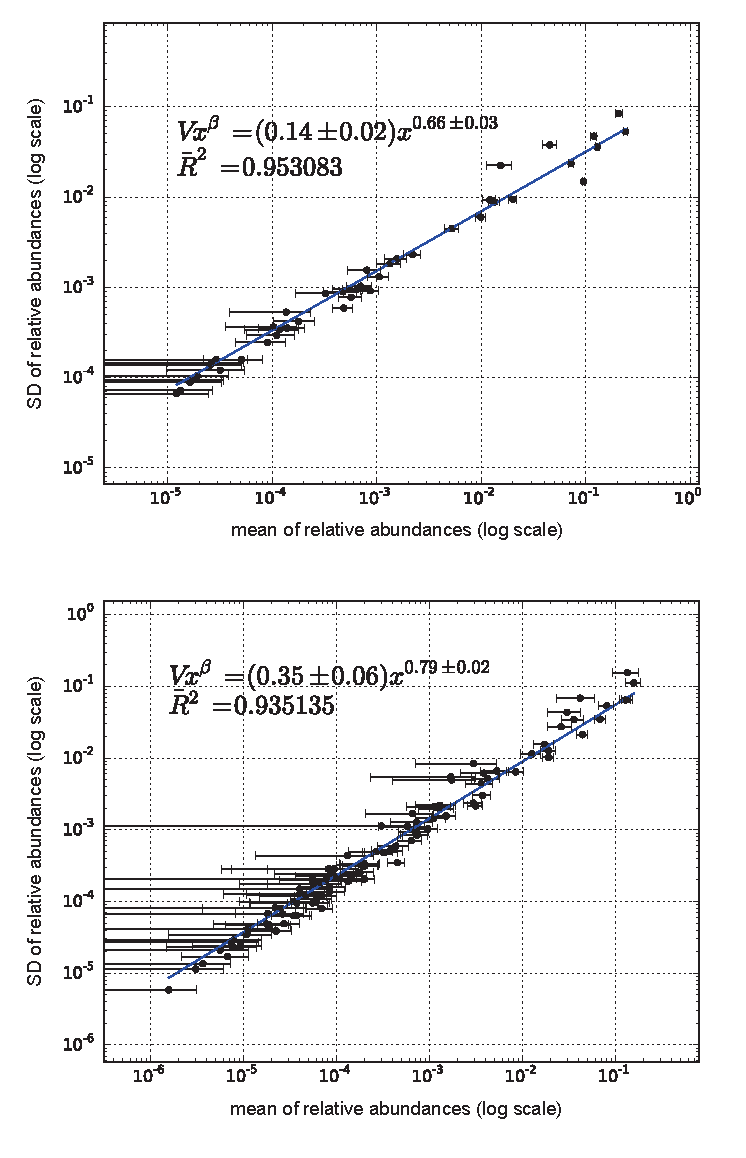
\includegraphics[width=0.7\textwidth]{figs/Fig1.eps}
	\caption{X-weighted power-law fits of the standard deviations versus the mean values for each bacterial genus monitored over time. The fit is shown for samples from a healthy subject (top) and from a subject diagnosed with irritable bowel syndrome (bottom), studied in our lab \cite{IBS}. Taylor's power law seems to be ubiquitous, spanning to six orders of magnitude. $V$ corresponds to the y-intercept and $\beta$ to the slope of the line. The error bars (\emph{mean-axis}) are the SEM.}
	\label{fig:main1}
\end{figure}

Taylor's parameters describing the temporal variability of the gut microbiome in our sampled individuals are shown in Supplementary Tables S\ref{tab:diet} to S\ref{tab:LEA}. Our results hint at ubiquitous behavior. Firstly, the variability (which corresponds to the maximum amplitude of fluctuations) was large, which suggests the resilient capacity of the microbiota. Secondly, the scaling index was always smaller than one, which means that more abundant taxa were less volatile than less abundant ones. In addition, Taylor's parameters for the microbiome of healthy individuals in different studies were compatible with estimated errors. This enabled us to define an area in the Taylor parameter space that we called the \emph{healthy zone}. 

In order to jointly visualize and compare the results of individuals from different studies\cite{IBS,moving,antibiotic,LEA,kwashiorkor,diet,hostlife}, their Taylor parameters were standardized, with standardization meaning that each parameter was subtracted by the mean value and divided by the standard deviation of the group of healthy individuals for every single study independently. Due to the different systematics in each study, we defined a healthy region for each one of them, standardized to mean zero and variance one and computed mean and variance of ?unhealthy? with this standardization (for details of the procedure, please see Standardization subsection in Material and Methods). Therefore, different studies were isolated so that individuals from a given study did not affect the results on the ?unhealthy? individuals of the other studies. We think this statistical approach was safer, as we avoided to combine data with very different systematic errors. The healthy zone and the standardized Taylor parameters for individuals whose gut microbiota was compromised (i.e., they were suffering from IBS, kwashiorkor, altered diet, intake of antibiotics, a Salmonella infection, or had gone on a trip abroad) are shown in Figure \ref{fig:main2}. The variability in children developing kwashiorkor was smaller than that of their healthy twins. A meat/fish-based diet significantly increased variability when compared to a plant-based diet. All other cases presented increased variability, which was particularly severe and statistically significant at over 95\% confidence level (CL), for grade III obese patients on a diet, individuals taking antibiotics, the subject who had a Salmonella infection, the subject who did a travel abroad or the IBS-diagnosed patients. One global property emerged from all the worldwide data collected: the Taylor's parameters characterized the statistical behavior of microbiome changes. Furthermore, we verified that our conclusions were robust to systematic errors as a result of taxonomic assignment (see Taxa level selection in Material and Methods).

\begin{figure}
	\centering
	%\includegraphics[width=0.9\textwidth]{results/finalplot11.pdf}
	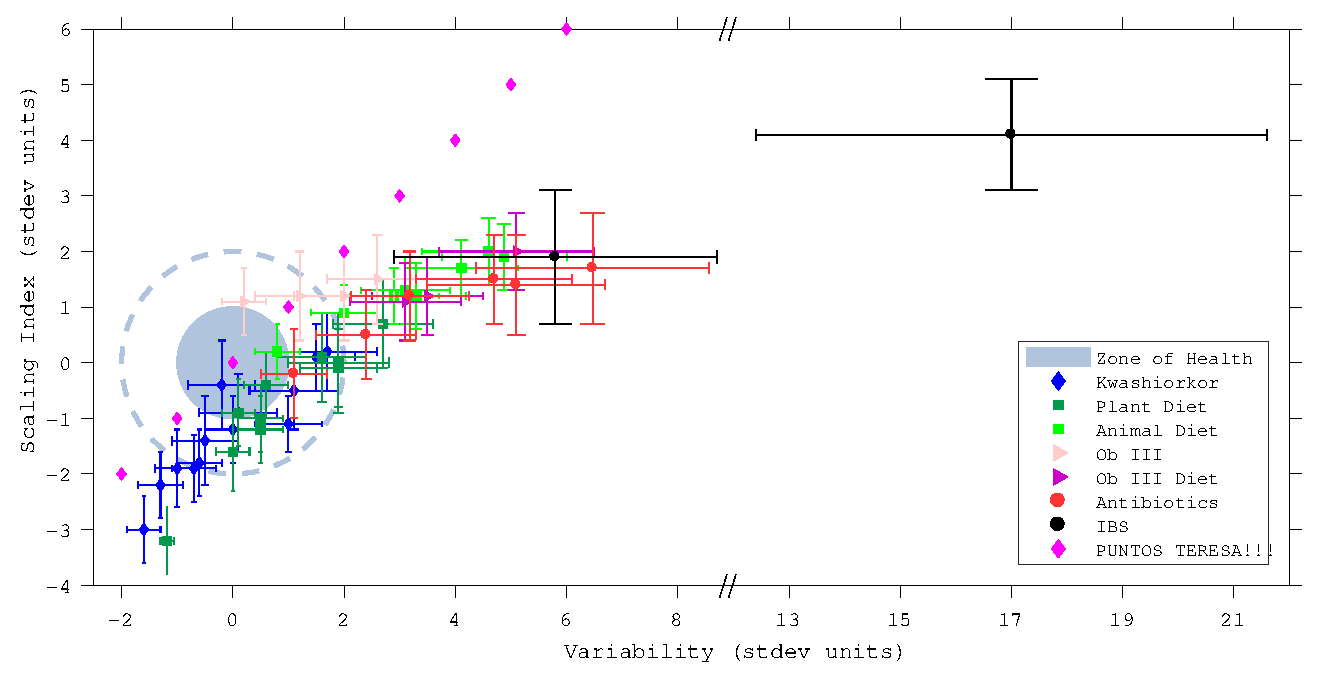
\includegraphics[width=1.0\textwidth]{figs/Fig2.eps}
	\caption{Taylor's law parameter space. All the data studied in this work were compiled here. The colored circle corresponds to a 68\% confidence level (CL) region of healthy individuals in the Taylor's parameter space, while the dashed line delimites the 98\% CL region. Points with errors place gut microbiome in the Taylor's parameter space, for each individual whose microbiota was compromised. It should be noted that the parameters were standardized (standard deviation units) to the healthy group in each study for every single study independently, for demonstrative and comparative purposes.}
	\label{fig:main2}
\end{figure}

Taylor's power law has been explained in terms of various effects, though none have brought a general consensus. It can be shown to have its origin in mathematical convergence which is similar to the central limit theorem, and thus virtually any statistical model designed to produce a Taylor law converges to a Tweedie distribution\cite{stat}, providing a mechanistic explanation based on the statistical theory of errors\cite{convergence1,convergence2,convergence3}. To reveal the generic mechanisms that drive different scenarios in the $\beta-V$ space, we modeled the system by assuming that taxon relative abundance followed a Langevin equation with, on the one hand, a deterministic term that captured the fitness of each taxon and, on the other hand, a randomness term associated with Gaussian random noise\cite{ranking}.Both terms were modeled by power laws, with coefficients that can be interpreted as the taxon fitness $F_i$ and the variability $V$ (see Model in Material and Methods). Fitness $F_i$ captures the time scale that the system needs to reach equilibrium (the size of variability $V$ may or may not allow to reach it). $F_i$ has dimensions of 1/time and roughly corresponds to the half-life of the system when decaying to the stable state. In fact, it is exactly the half-life if $\beta$ is one and $V$ is negligible. In this model, when $V$ is sufficiently low, abundances are stable in time. Differences in the variability $V$ can induce a noise-induced phase transition in the relative abundances of taxa. The temporal evolution of the probability of a taxon having the abundance $x_i$, given its fitness, is governed by the Fokker--Planck equation. The results of solving this equation show that stability is best captured by a phase space determined by the fitness $F$ and the amplitude of fluctuations $V$ (see Figure \ref{fig:main3}).

\begin{figure}
	\centering
	\vspace*{-5mm} % Corrects overbox of the figures
	%\includegraphics[width=0.8\textwidth]{results/finalPlot33_new.pdf}
	\includegraphics[width=0.8\textwidth]{figs/Fig3.eps}
	\caption{Microbiota states can be placed in the phase space $F-V$. The light-blue shaded region corresponds to the stable phase, while the grey shaded region is the unstable phase (the phase transition line is calculated for  $\alpha$ = $\beta$ = 0.75). We placed healthy individuals (green) and individuals whose gut microbiota is threatened (antibiotics, IBS) in the phase space fitness--variability. The gut microbiota of healthy individuals over a long term span show a quasi--periodical variability (central period is ten days). We show that taking antibiotics (AB1 and AB2 correspond to the first and second treatment, respectively) induces a phase transition in gut microbiota, which impacts on future changes. We also show an IBS--diagnosed patient transiting from the unstable to the stable phase.}
	\label{fig:main3}
\end{figure}

The model predicted two phases for the gut microbiome: a stable phase with large variability that enabled some changes in the relative abundances of taxa; and an unstable phase with even larger variability, above the phase transition, where the order of abundant taxa varies significantly over time. The phase transition is continuous (of second order), as is the crossing of the boundary. The state variable is the composition. Any disturbance modifies the composition of the microbiota, with different compositions encoding different $F$ and $V$. Our model can be solved analytically, which allows to a simple understanding of the different regimes, and in particular, to calculate the formula of the transition region. If $V$ is sufficiently small compared to $F$, there is a maximum in the likelihood in the physical region (relative compositions larger than zero and smaller than one), i.e., there is a best composition solution of the differential equation, which is the ordered solution. On the contrary, if $V$ is sufficiently large compared to $F$ the maximum in the likelihood is outside the physical region, i.e., the best composition solution of the differential equation is at the boundaries (either zero or one) and all physical solutions have comparable likelihoods, which is the noisy phase. The microbiome of healthy individuals was found to be in the stable phase, while the microbiome of several other individuals was shown to be in the unstable phase. In particular, individuals taking antibiotics and the IBS--diagnosed patient \emph{P2} had the most severe symptoms. In this phase diagram, each microbiota state is represented by a point at its measured variability $V$ and inferred fitness $F$. The model predicted high average fitness for all taxa, i.e., taxa were narrowly distributed in $F$. The fitness parameter was chosen with different values for demonstrative purposes. Fitness was larger for the healthiest subjects and smaller for the IBS--diagnosed patients.

%%%
\subsection*{Rank stability of the taxa} 

The rank dynamics and stability plots in Figure \ref{fig:corrank_HLS_abroad} and \ref{fig:corrank_HLS_returned} show the variations in rank over time for the most dominant taxa and their calculated Rank Stability Index (RSI, as discussed in Material and Methods) for the gut microbiome taxa of a healthy subject, the individual \emph{A} in the host lifestyle study \cite{hostlife}. The Figure \ref{fig:corrank_HLS_abroad} covers the period when the individual is travelling abroad and the Figure \ref{fig:corrank_HLS_returned} covers the subsequent period. The taxa were listed ordered by their accumulated frequency over the time series, with the y-axis being the overall dominance axis for each sample set. Generally speaking, we observed that the most dominant taxa had the highest rank stability. 

\begin{figure}
	\centering
	%\vspace*{-10mm} % Corrects overbox of the figures
	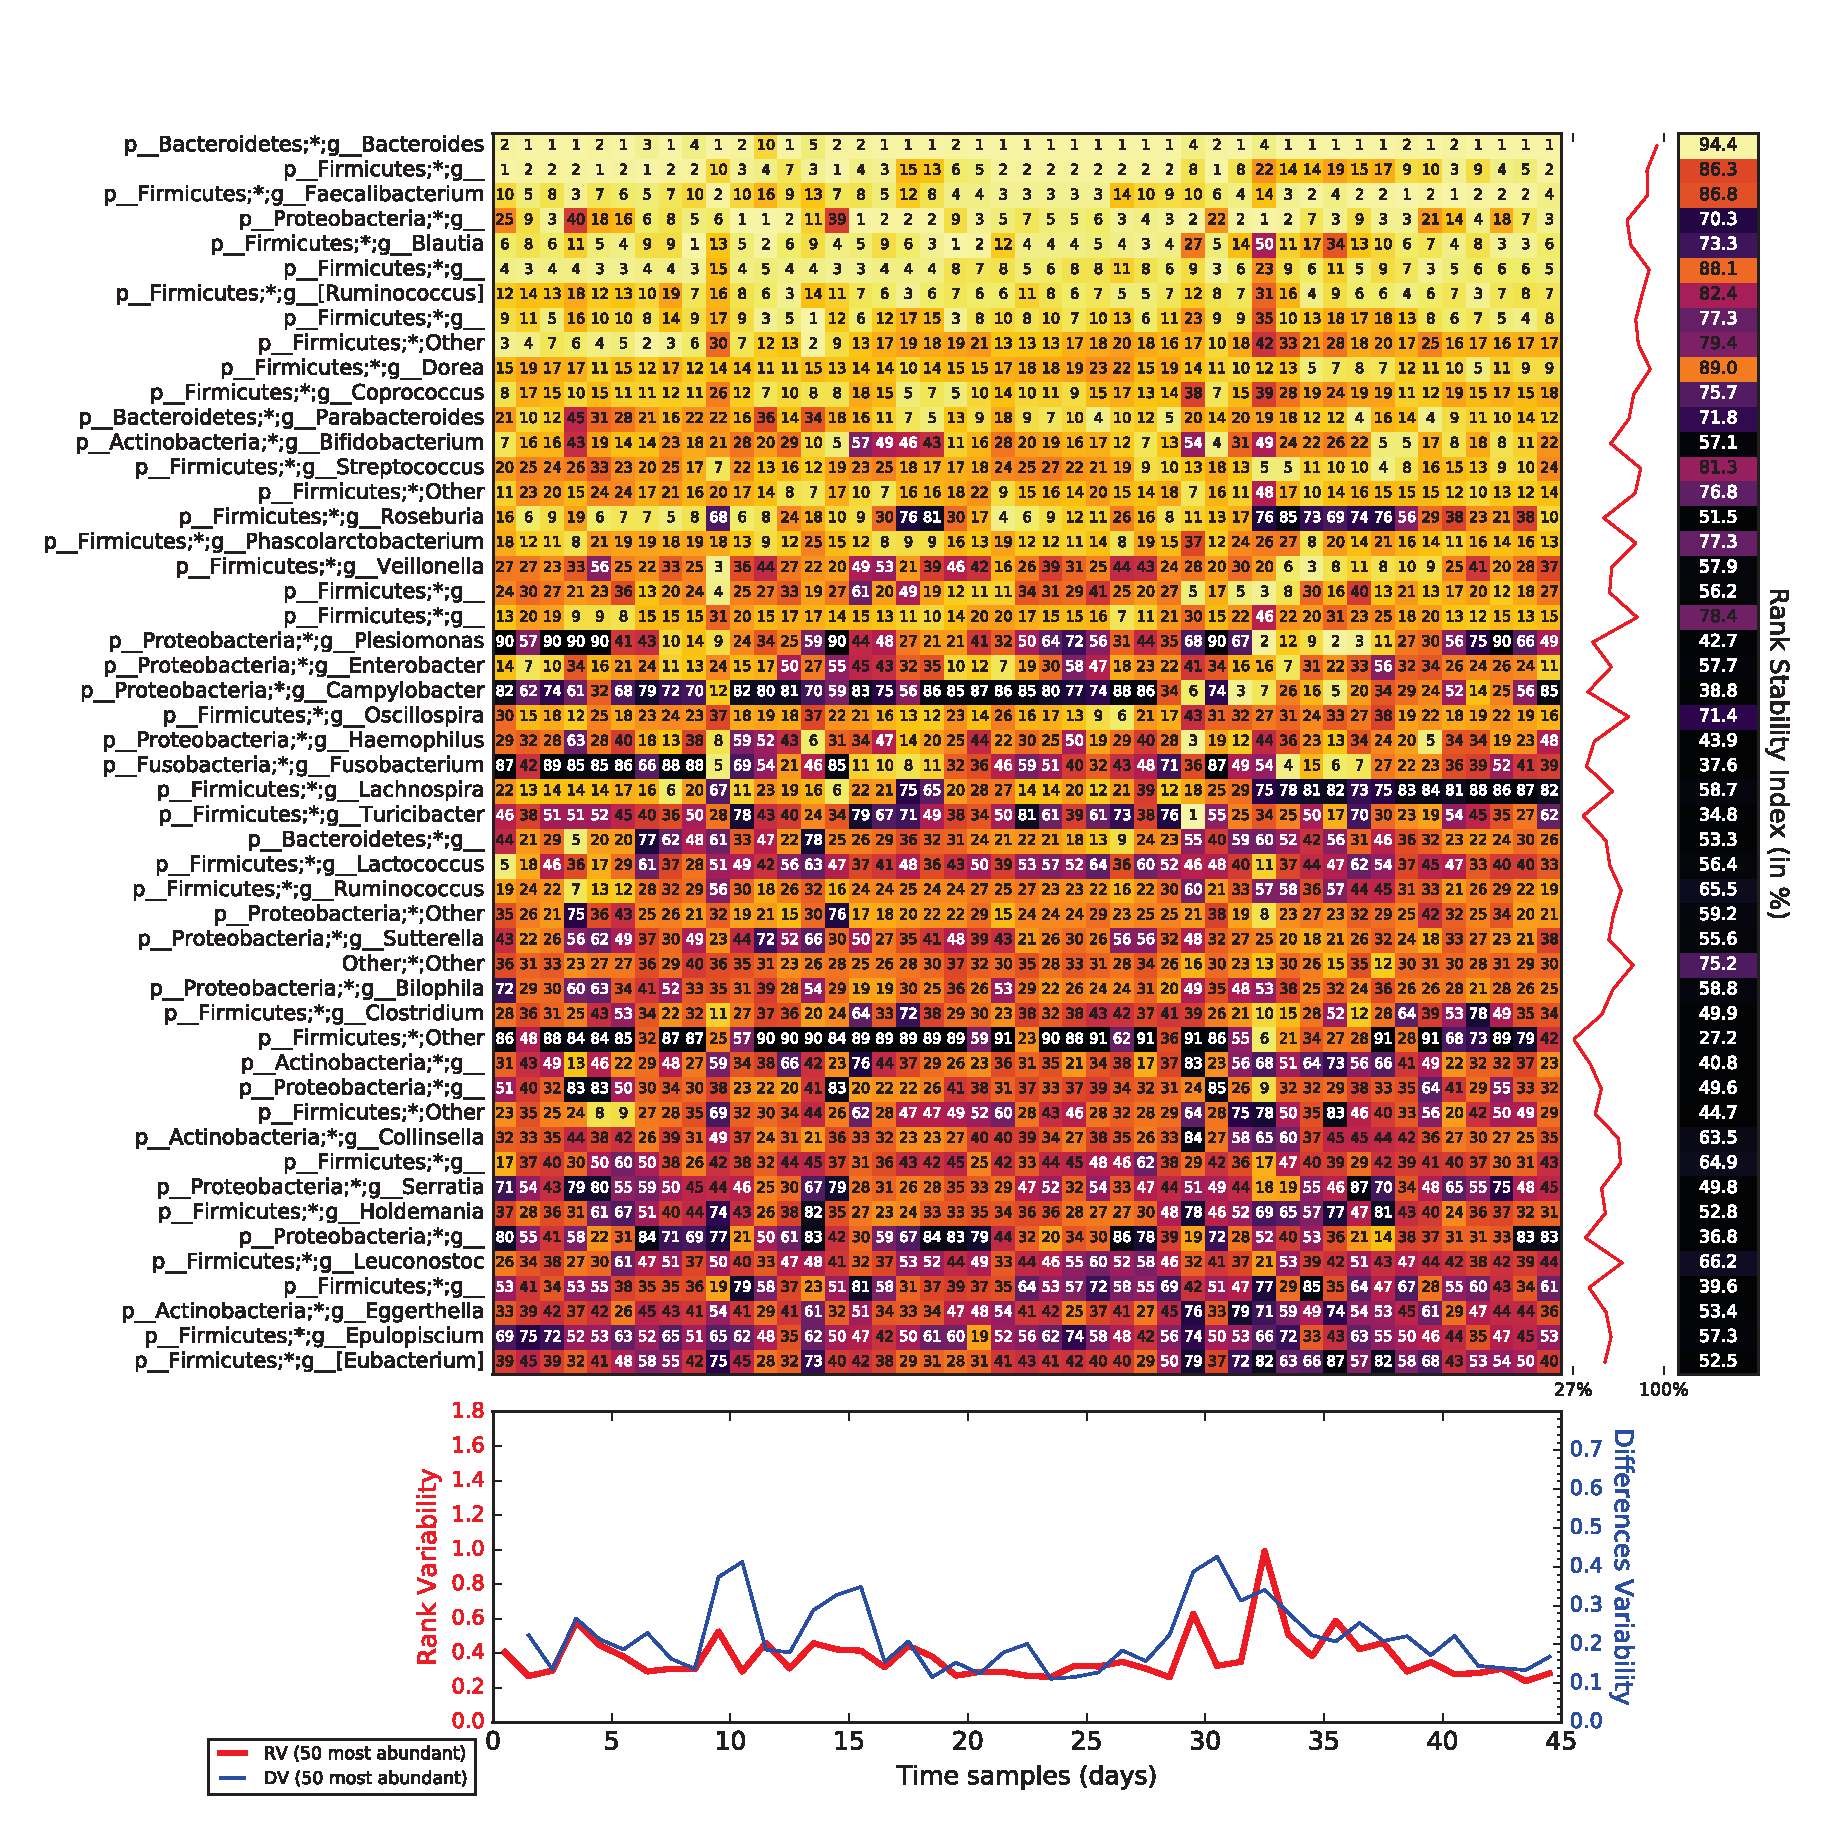
\includegraphics[width=1.0\textwidth]{figs/Fig4.eps}
	\caption{Rank variation over time for the 50 most dominant elements (taxa) and their calculated RSI (Rank Stability Index), Rank Variability (RV) and Differences Variability (DV), as detailed in Rank stability and variability in Material and Methods, for a special period (days 72 to 122, travelling abroad) belonging to the individual \emph{A} in the host lifestyle study \cite{hostlife}.}
	\label{fig:corrank_HLS_abroad}
\end{figure}

\begin{figure}
	\centering
	%\vspace*{-10mm} % Corrects overbox of the figures \hspace*{-4.5mm}
	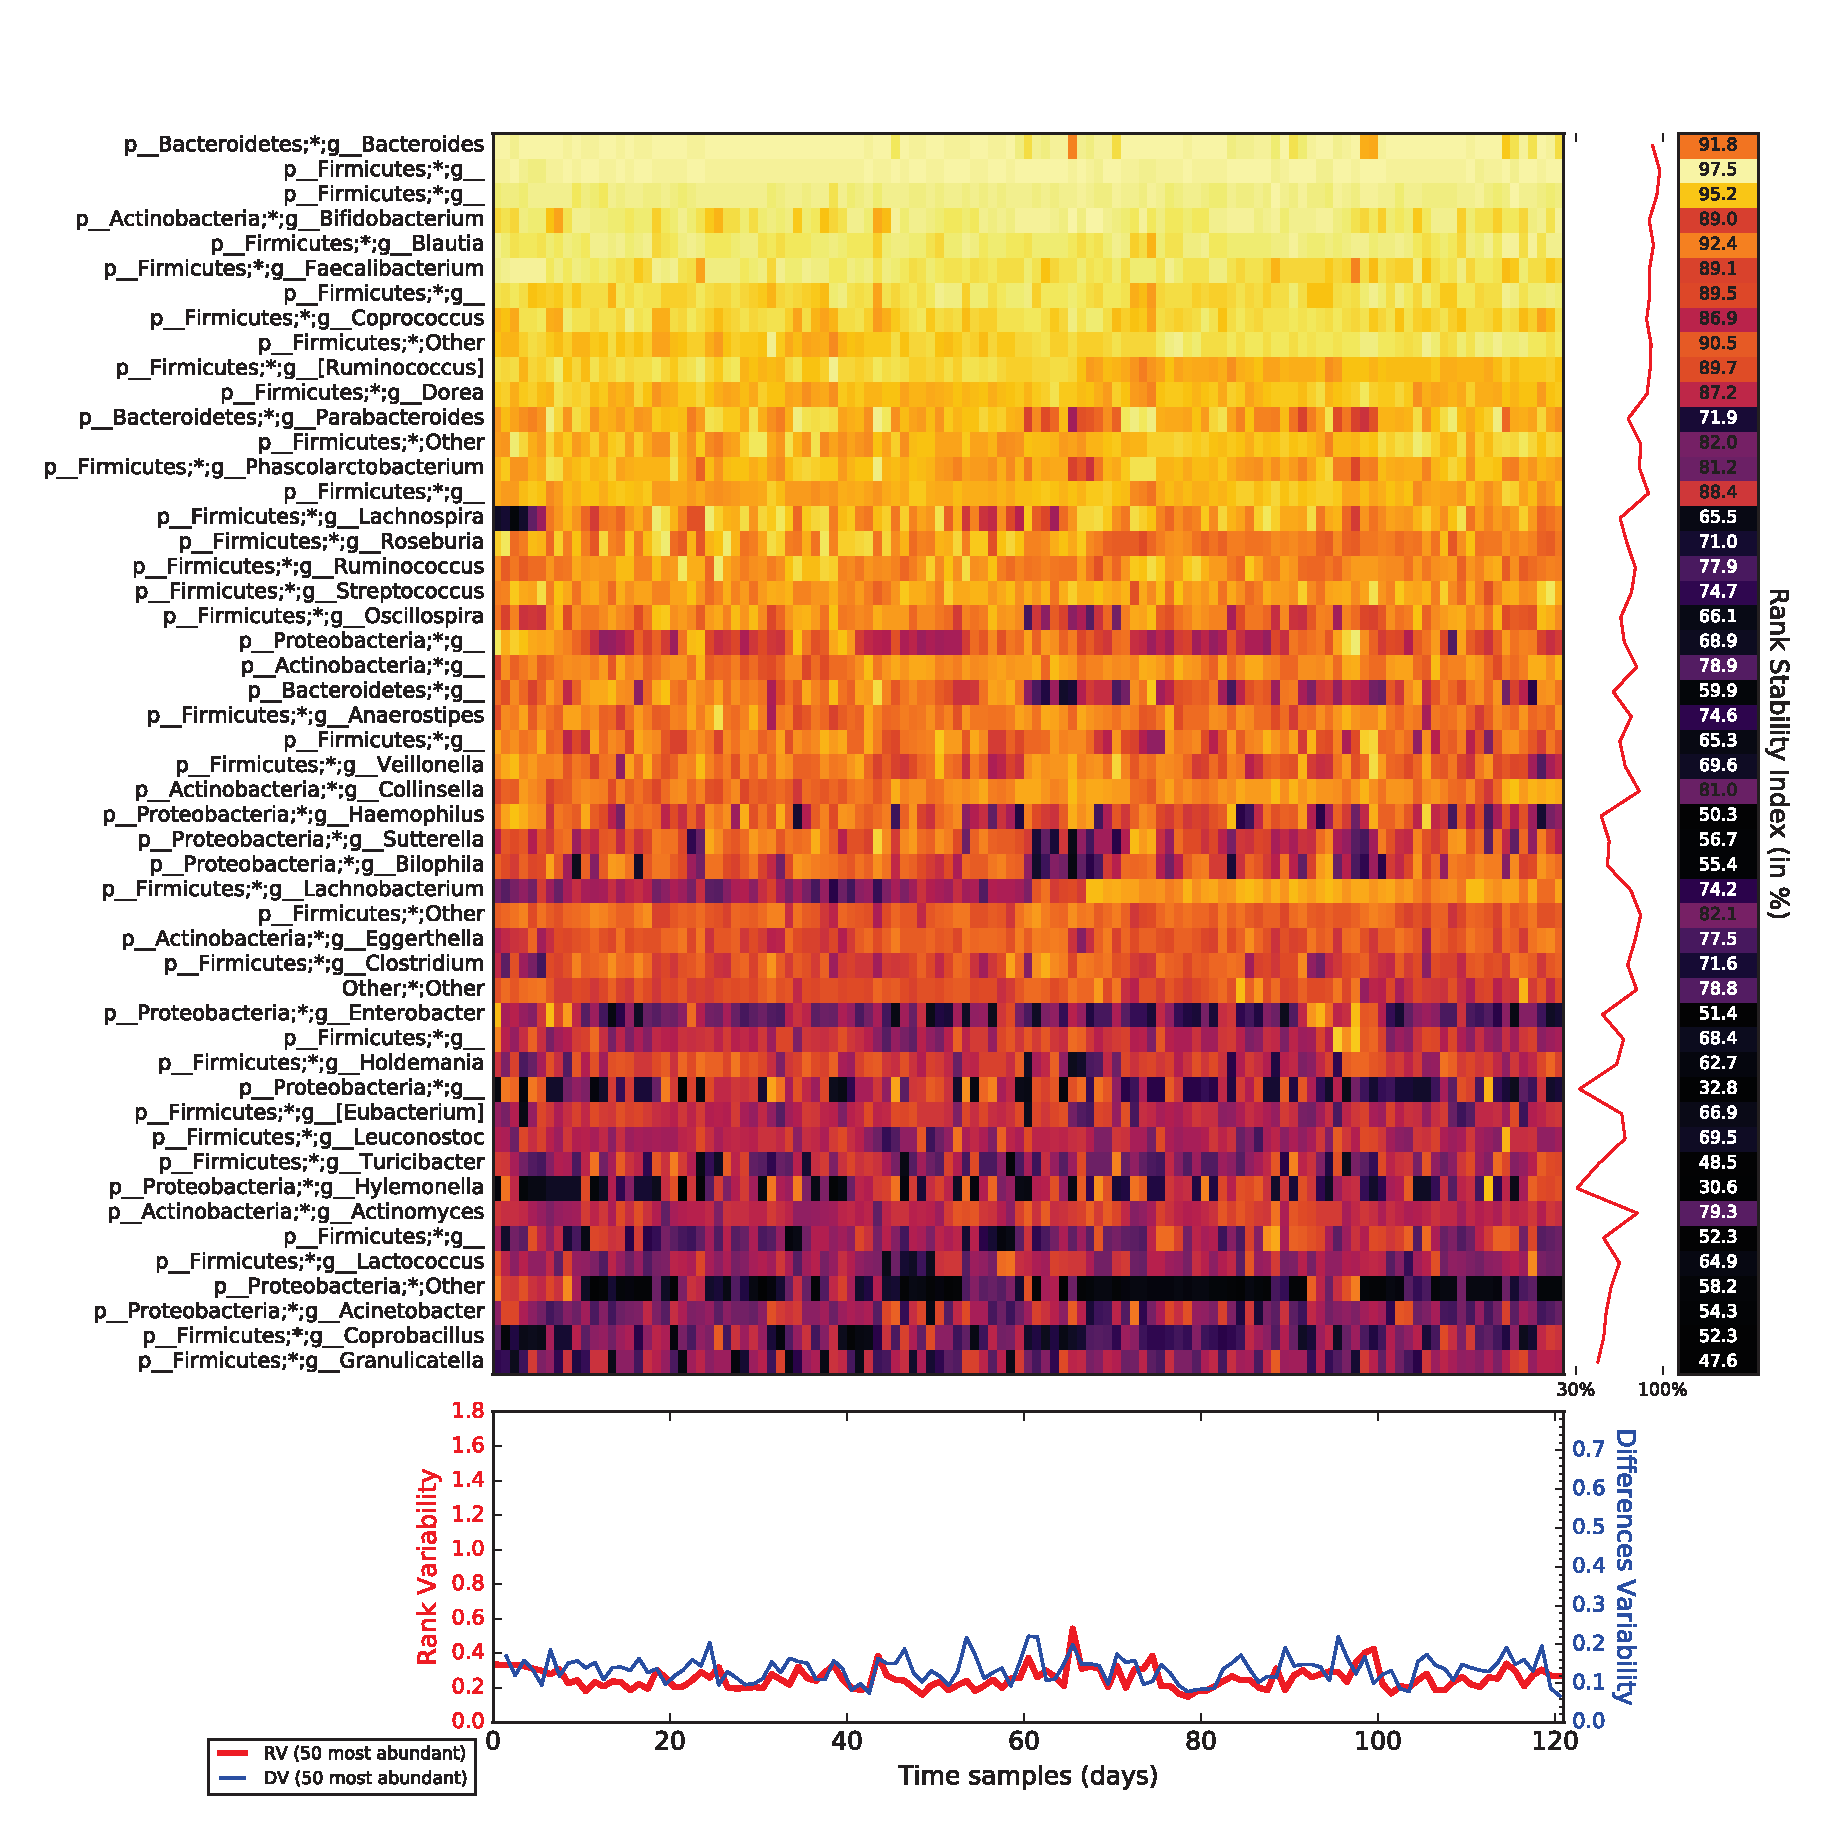
\includegraphics[width=1.0\textwidth]{figs/Fig5.eps}
	\caption{Rank variation over time for the 50 most dominant elements (taxa) and their calculated RSI (Rank Stability Index), Rank Variability (RV) and Differences Variability (DV), as detailed in Rank stability and variability in Material and Methods, for an ordinary period (days 123 to 256, after the trip) belonging to the individual \emph{A} in the host lifestyle study \cite{hostlife}.}
	\label{fig:corrank_HLS_returned}
\end{figure}

For the trip abroad in Figure \ref{fig:corrank_HLS_abroad}, beyond the differences in dominance for the particular taxa, we still observed that the most dominant were the most rank stable. Moreover, the medium-ranked taxa were quite rank unstable, mostly due to transient (often one or two consecutive samples) yet dramatic drops in their relative abundance, which usually occurred more than twice during their time series.

Nevertheless, in the particular case of the next period, the one subsequent to the trip, in Figure \ref{fig:corrank_HLS_returned}, some taxa showed higher stability than other more dominant taxa, forming a kind of \emph{rank stability islands} for medium--ranked taxa, since they show a moderately stable index (RSI roughly over 70\%). In particular, this is the case for the genera \emph{Actinomyces}, \emph{Leuconostoc}, \emph{Lachnobacterium}, \emph{Eggerthella}, \emph{Clostridium} and	\emph{Collinsella}. For those genera, both the overall rank and the RSI were clearly lower during the trip (RSI under 70\%). \emph{Actinomyces} and \emph{Lachnobacterium} are even not shown in Figure \ref{fig:corrank_HLS_abroad} because they sank to positions 56 and 77, respectively. On the contrary, \emph{Leuconostoc} was the least sensitive to the change of lifestyle. In addition, it is worth mentioning that \emph{Lachnobacterium} showed anti-correlation over time against the vast majority of the taxa classified in this study.

We also found those \emph{rank stability islands} for medium-ranked taxa in the other periods belonging to the individual \emph{A} in the host lifestyle study \cite{hostlife} (see Supplementary Figure S\ref{supfig:corrank_HLS_before} and Supplementary Figure S\ref{supfig:corrank_HLS_after} for the corresponding rank plots). See Supplementary Table S\ref{tab:HLS_RSI} for details about the rank and RSI for the above-mentioned taxa over the different periods considered.

\begin{supfig}
	\centering
	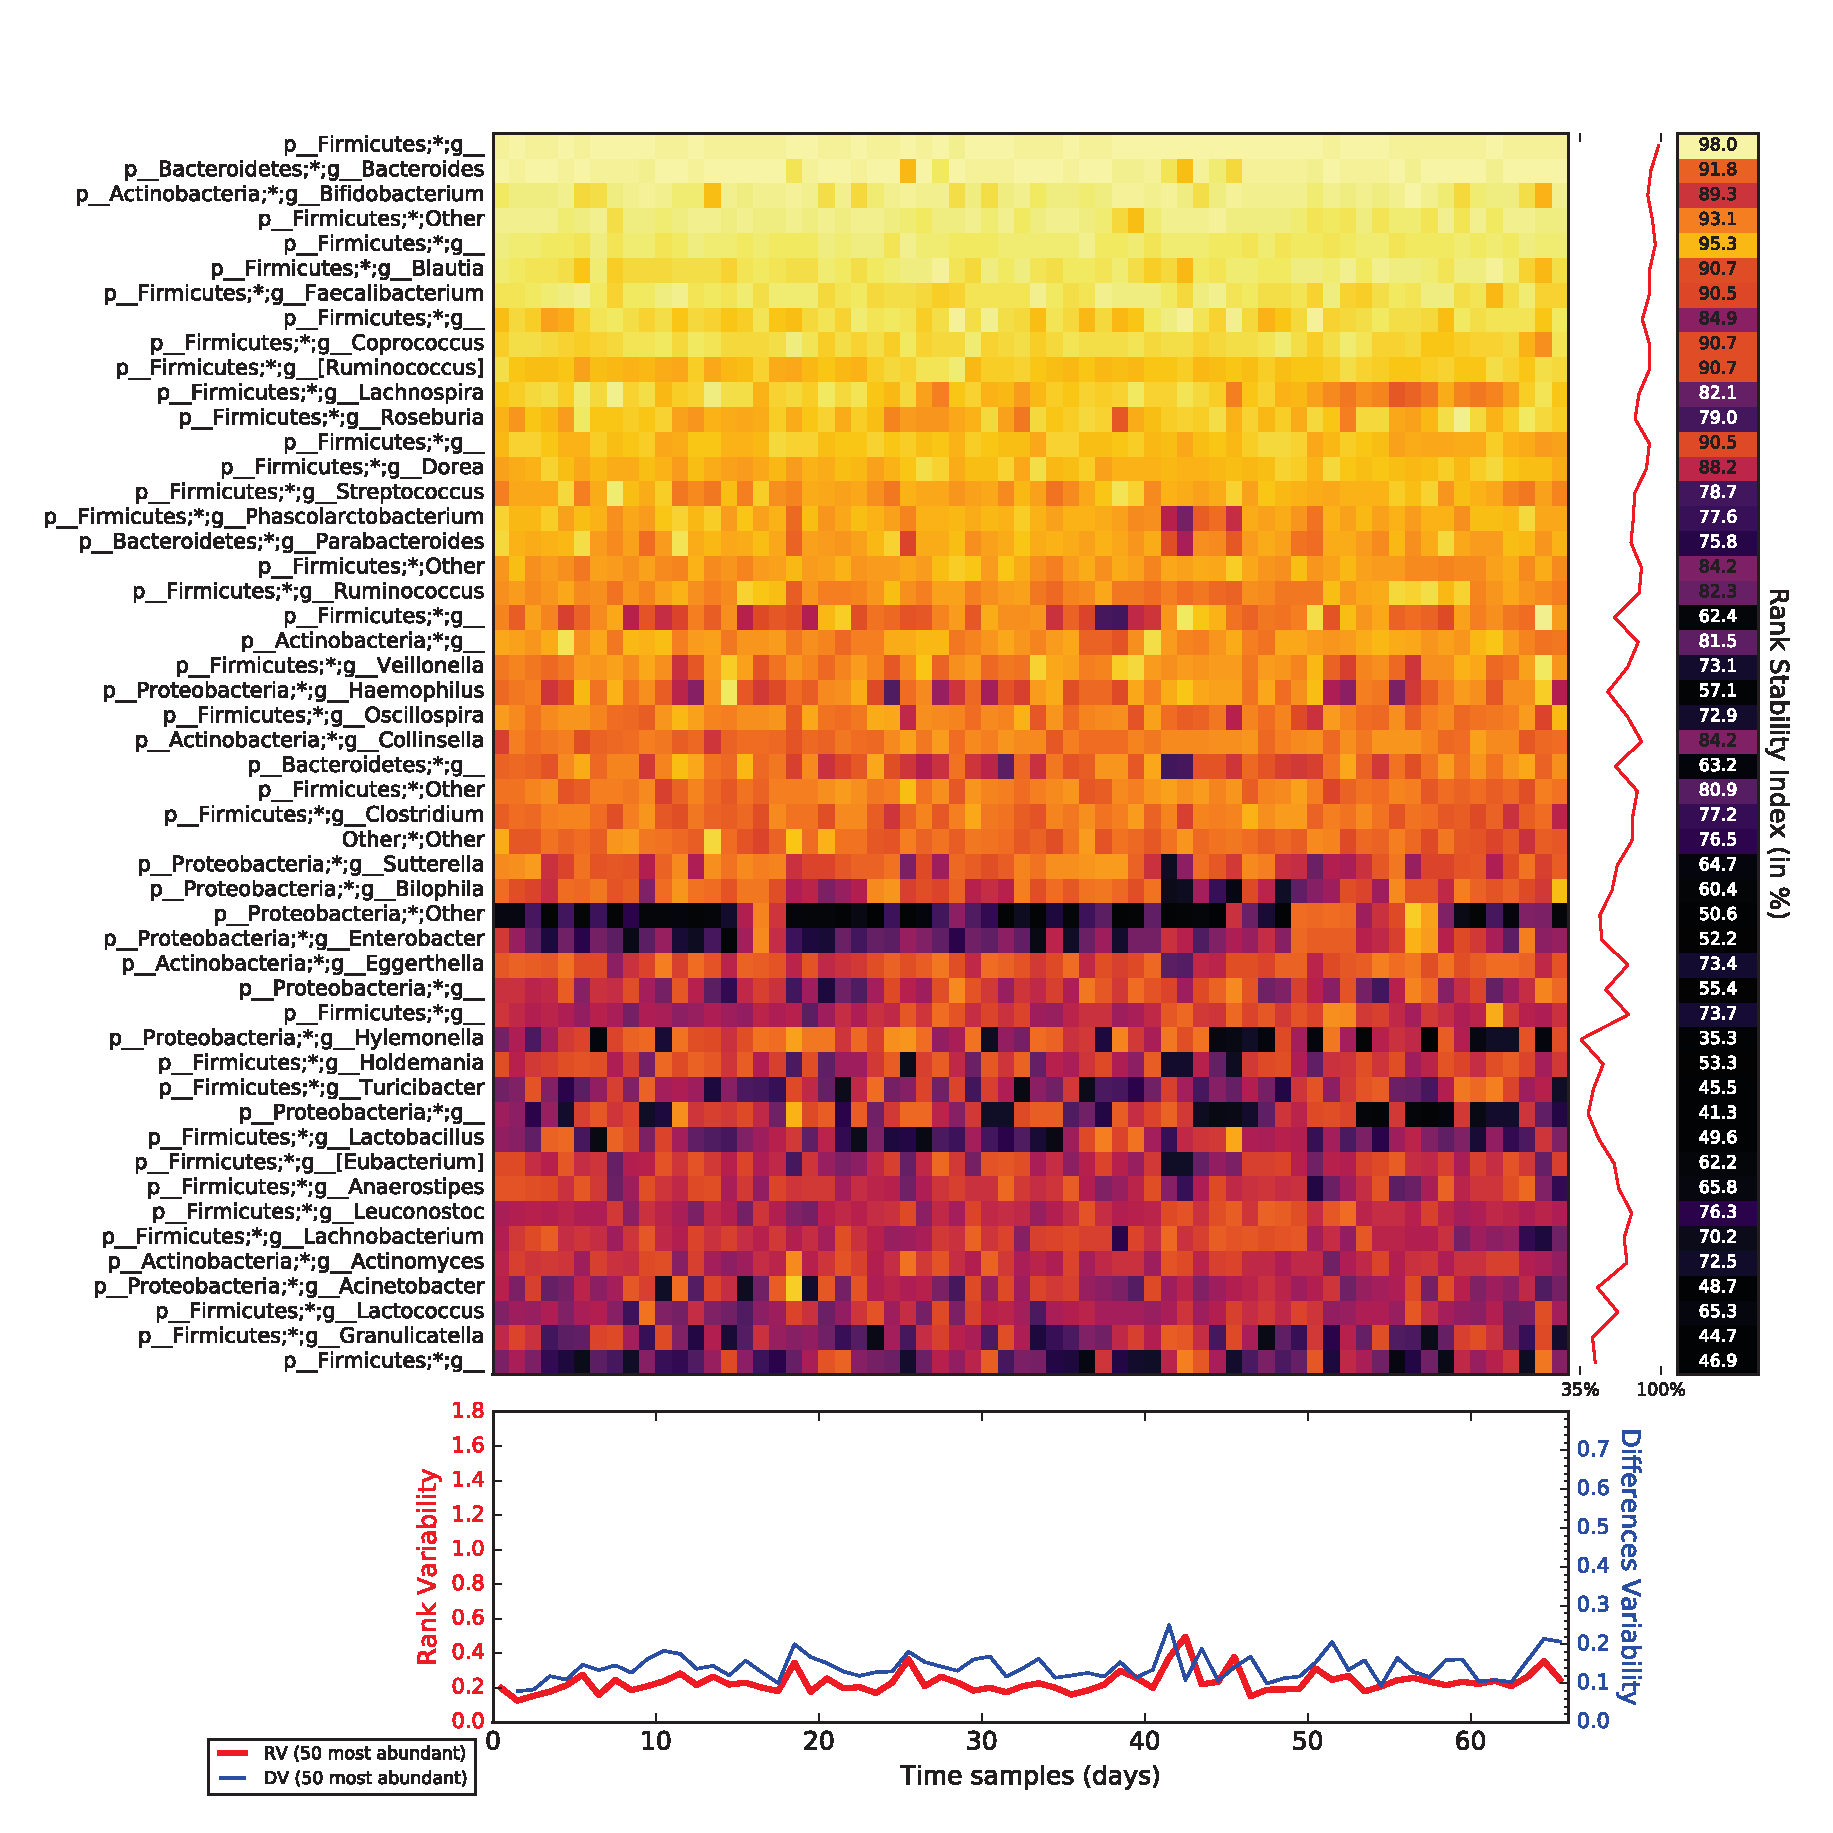
\includegraphics[width=1.0\textwidth]{figs/supfig_corrank_HLS_StoolA_before.eps}
	\caption{Rank variation over time for the 50 most dominant elements (taxa) and their calculated RSI (Rank Stability Index), Rank Variability (RV) and Differences Variability (DV), as detailed in Rank stability and variability in Material and Methods, for an ordinary period (days 0 to 70, before the trip) belonging to the individual \emph{A} in the host lifestyle study \cite{hostlife}.}
	\label{supfig:corrank_HLS_before}
\end{supfig}

\begin{supfig}
	\centering
	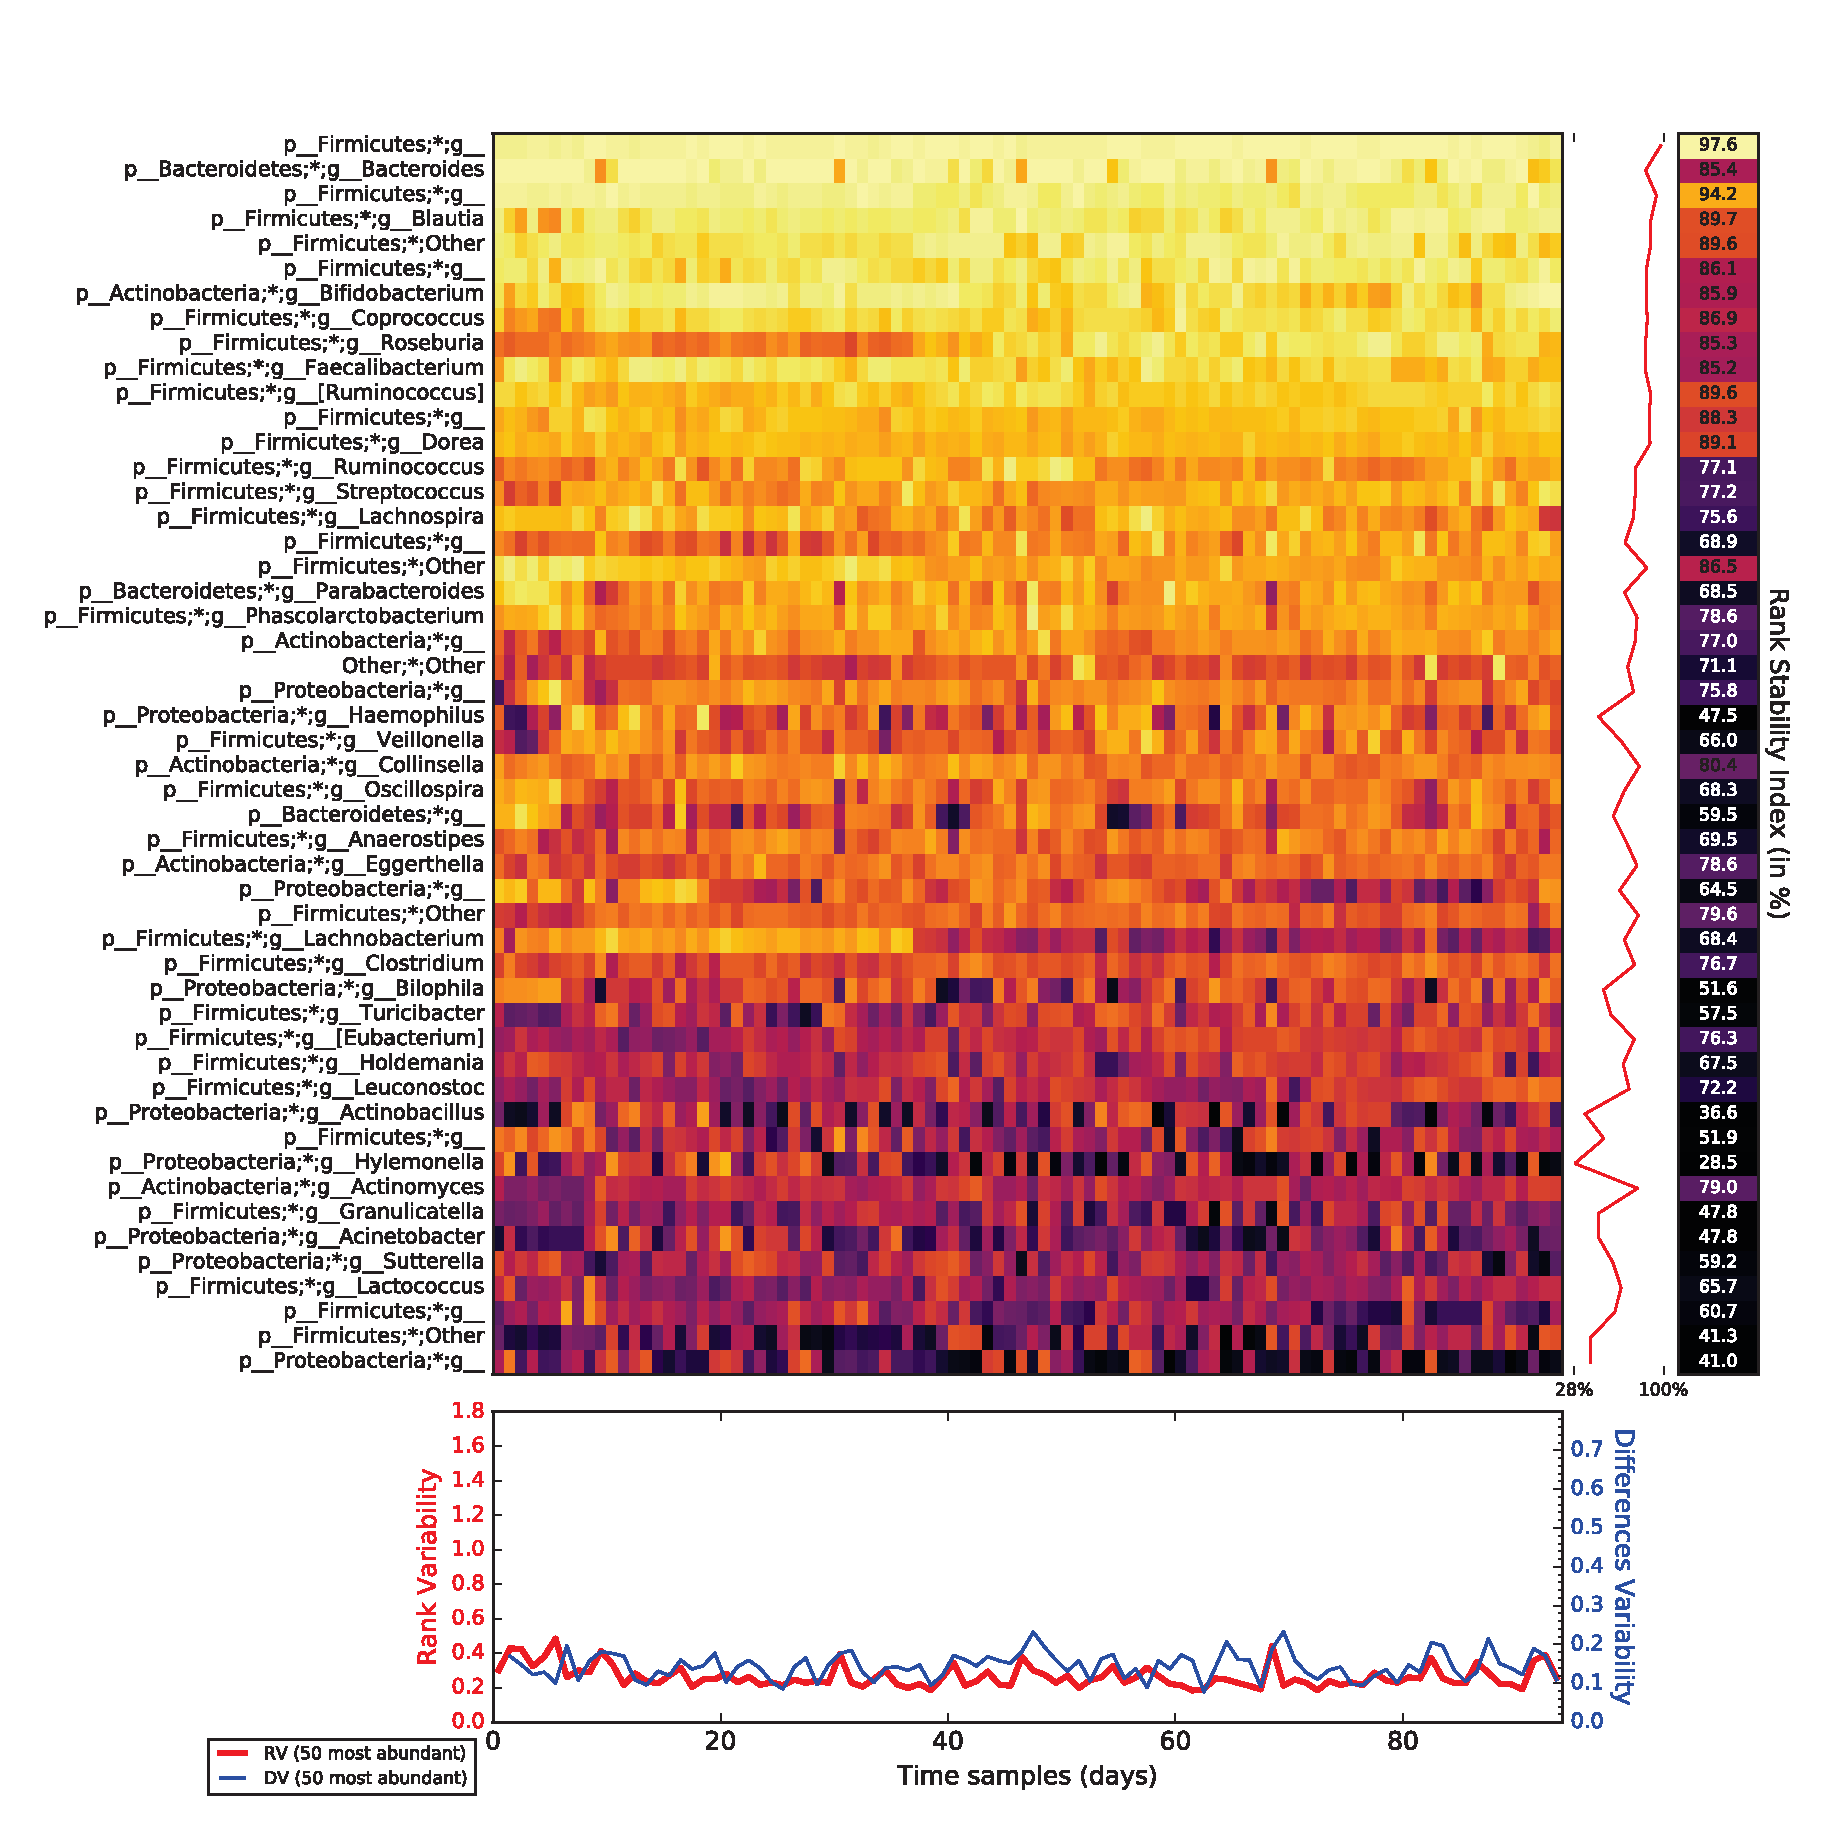
\includegraphics[width=1.0\textwidth]{figs/supfig_corrank_HLS_StoolA_after.eps}
	\caption{Rank variation over time for the 50 most dominant elements (taxa) and their calculated RSI (Rank Stability Index), Rank Variability (RV) and Differences Variability (DV), as detailed in Rank stability and variability in Material and Methods, for an ordinary period (days 257 to 364, further after the trip) belonging to the individual \emph{A} in the host lifestyle study \cite{hostlife}.}
	\label{supfig:corrank_HLS_after}
\end{supfig}

%%%
\subsection*{Time dependence of model parameters}

Finally, we studied the time dependence of the variability $V$ and power law index $\beta$ (see Model in Material and Methods) by using a sliding window approach. The total number of time points was divided into subsets of five points, where the following subset was defined by adding the next time sampling and eliminating the earliest one. Both parameters were calculated for each subset against the average time lapse. Figure \ref{fig:tempevo1} shows the variability $V$ as a function of time for the two individuals in Caporaso's study\cite{moving} corresponding to the gut microbiota of a male (upper plot) and a female (lower plot). Both samples showed changes in the variability $V$ with quasi--periodic behavior peaking at about 10 days. Variability grew more for the gut microbiota of the male and shared a minimal value of around 0.1 with the gut microbiota of the female. 

Figure \ref{fig:tempevo2} shows the time evolution of $V$ for patient \emph{P2} in the IBS study\cite{IBS} (upper plot) and patient \emph{D} in the antibiotics study\cite{antibiotic} (lower plot). The variability of the gut microbiota of \emph{P2} decreased from over 0.3 to below 0.2, showing a slow tendency to increase the order of the system.  Antibiotic intake led to a quick increase in variability which lasted for a few days to recover ordering. The second antibiotic treatment showed some memory traits (lower increase of variability) with a slower recovery. 

\begin{figure}
	%\includegraphics[width=1.0\textwidth]{results/sliwin/male_mov.pdf}
	%\hspace*{3mm}\includegraphics[width=0.448\textwidth]{results/sliwin/female_mov.pdf}
	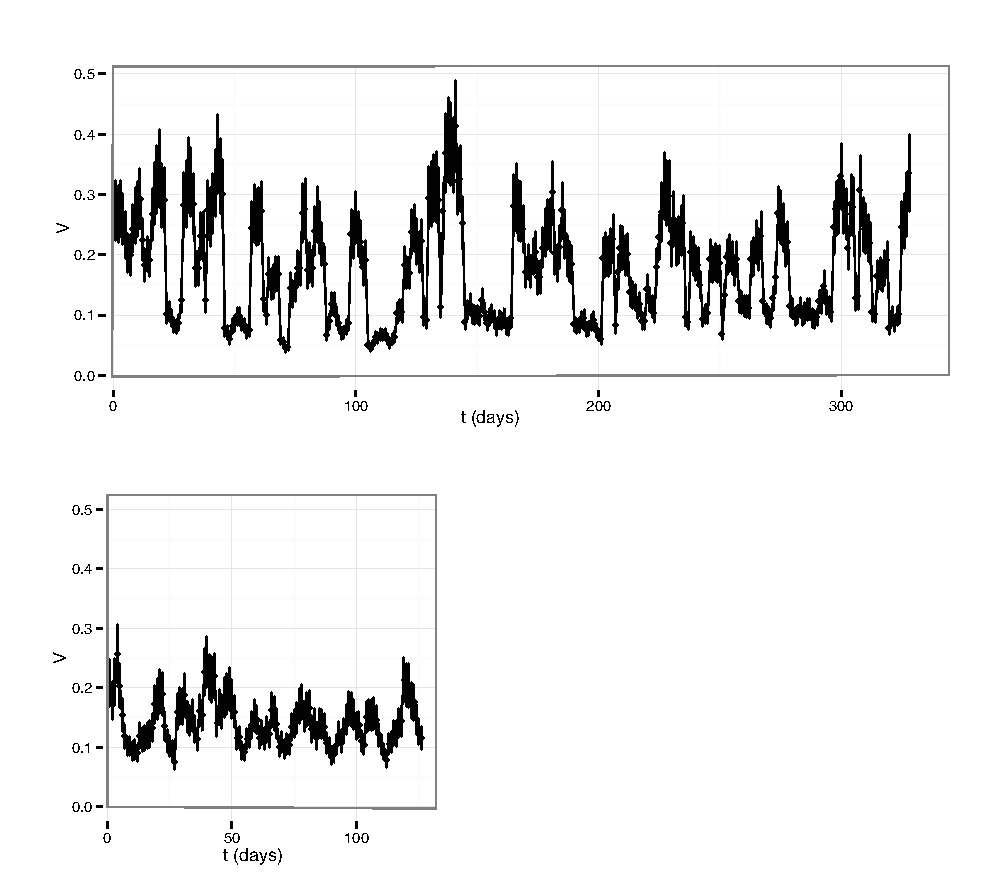
\includegraphics[width=0.99\textwidth]{figs/Fig6.eps}
\caption{$V$ as a function of time for the two individuals in Caporaso's study\cite{moving}: samples of gut microbiome of a male (upper plot) and a female (lower plot).}
\label{fig:tempevo1}
\end{figure}

\begin{figure}
	\centering 
 	%\includegraphics[width=0.8\textwidth]{results/sliwin/patP2_IBS.pdf}
  	%\includegraphics[width=1.0\textwidth]{results/sliwin/patD_antibio.pdf} 
	\includegraphics[width=0.99\textwidth]{figs/Fig7.eps}	
\caption{$V$ as a function of time for patient \emph{P2} in the IBS study\cite{IBS} (upper plot) and patient \emph{D} in the antibiotics study\cite{antibiotic} (lower plot). The blue vertical lines in the lower plot show the periods of antibiotic treatment.}
\label{fig:tempevo2}
\end{figure}

%\clearpage
%%% Discussion
\section*{Discussion}
% !TeX root = ./mSys_MAIN_rev2.tex
One of the highlights of this study is that is shows, independently of its condition, that microbiota follows Taylor’s law. We have seen that in each case the value of the scaling index is always less than the unity (using standard deviation as the dispersion measurement), which provides us with information about the community structure. This means that, in relative terms, the most abundant elements in the population are less volatile to perturbations than the less abundant ones. The explanation for this universal pattern is not clear although some hypotheses have been tested in other studies, such as the presence of negative interactions in the population \cite{kilpatrick}, and a demonstration that this may depend on reproductive correlation \cite{ballantyne}. Nevertheless, none of these explanations are sufficient when it comes to microbiota, as the term reproduction is diffuse the interactions between its components are not only based on competition \cite{joao, mehta, bucci}. Moreover, even such negative interaction may not effectively yield values less than the unity when referring to a bacterial species (41). Nonetheless, the values obtained in all cases were very similar to each other, which may suggest that the community structure is preserved throughout the different scenarios studied herein.

The second parameter provides information about noise and can be directly linked to the variability or fluctuation amplitude of the population over time. It is a direct estimator of the stability of the system under study. As we have shown above, the healthy subset of each study has lower variability than the non-healthy subset, when dealing with adult subjects. Interestingly, the variability parameter was higher in the healthy subset in the study of discordant twins suffering from kwashiorkor disease \cite{kwashiorkor}. In this respect, research has shown that infant microbiota needs to develop toward a definite, adult state \cite{koenig}. This implies that temporal variability is greater in children than in a healthy adult, which should be temporally stable. Thus, our results could indicate this variability is necessary in order to reach that adult state. Furthermore, as we wanted to see how this variability shifted over time, we calculated the changes in this parameter for the samples which had enough time sampling. As shown in Figure \ref{fig:tempevo1}, the variability of microbiota fluctuated over time. Interestingly, Figure \ref{fig:tempevo2} shows how this parameter reflected the two antibiotic intakes in one of the patients in the study by Dethlefsen and Relman \cite{antibiotic} particularly the apparent resilience of the microbiota due to the reduced increase in variability during the second antibiotic intake.

The primary hypothesis of this work is that, in adults, having a healthy microbiota means that the microbial population is stable over time.  This stability means the microbiota does not shift and become susceptible to external or internal perturbations causing dysbiosis. In order to use the valuable information provided by the empirical law of Taylor’s work, herein we have proposed the use of Langevin’s equation to model how stability ranking changed  over time. While the system noise component can be directly measured as its variability, the other main term needs to be inferred from the model. This term, which we have named "fitness", enables the system to remain stable when confronted with potential perturbations. In ecological terms, this could represent the nature of interactions present among bacteria, between bacteria and other minority populations, such as fungi or archaea, between bacteria and the viral component in microbiota, and interactions between the host and the whole microbiota. As this is a first step to model the temporal stability of microbiota, and given its complex nature, we calculated fitness using the Fluctuation Dissipation Theorem as a first approximation \cite{FD}. Thus, future works are required to model the fitness of microbiota in order to provide a more accurate model with higher predictive power. 

By solving Langevin’s differential equation, we obtain a phase diagram where each microbiota sample can be placed by its fitness and variability into one of two phases, according to the stability ranking of the system. As shown by the phase--space in Figure \ref{fig:main3}, three different conditions can occur. The first is a healthy microbiota with some fluctuations, as shown by one of the subjects in Caporaso \emph{et al.}'s study \cite{moving}. Because this case would have good fitness, its temporal variability would not place the microbiota in the unstable phase of the diagram. Secondly, we have a subject from the study by Dethlefsen and Relman \cite{antibiotic} whose microbiota was perturbed twice by an antibiotic intake, undergoing sufficient change so as to lose its stability, and hence be placed in the unstable part. In this location, it is more sensitive to potential perturbations such as, for example, opportunistic infections. In the third and last condition, the subject was already in the unstable phase due to a health issue, i.e. IBS. This can be observed in one of the patients in Durban \emph{et al.} \cite{IBS}. In addition, it was shown that this subject’s health status improved during the experiment, implying that his/her microbiota also recovered stability. Interestingly, in the study made by David \emph{et al.} \cite{hostlife} the subject who had a Salmonella infection during the experiment underwent a significant shift in variability with eventual recovery from the perturbed state (see Supplementary Figure S\ref{supfig:HLS_xWSummary}).

\begin{supfig}
	\centering
	%\vspace*{-10mm} % Corrects overbox of the figures
	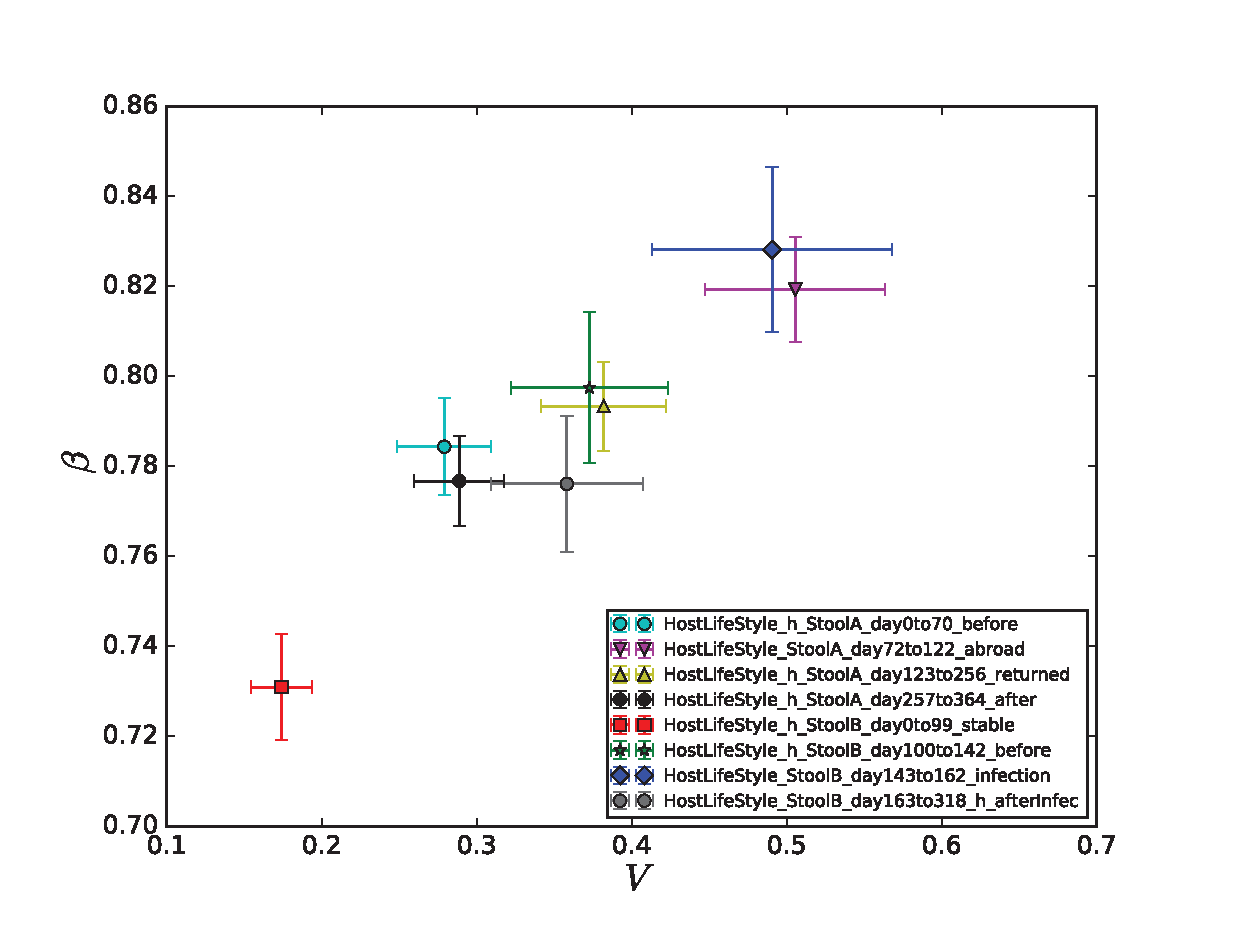
\includegraphics[width=0.99\textwidth]{figs/supfig_HLS_xWSummary.eps}
	\caption{Taylor's law parameter space for intervals concerning gut microbiota in the host lifestyle study\cite{hostlife}. We observe that subject \emph{B}, who suffered a Salmonella infection during the experiment, had a relevant shift in the parameters from \emph{\_before} to \emph{\_infection} and a final recovery from the perturbed state to \emph{\_afterinfec}, which lies in the parameter area compatible with the healthy and stable intervals (see Supplementary Table S\ref{tab:Ab-IBS-HLS}). Subject \emph{A} also had a shift in variability from \emph{\_before} to \emph{\_abroad} and back to \emph{\_returned}, also in the proximity zone of healthy and stable periods.}
	\label{supfig:HLS_xWSummary}
\end{supfig}
 
Specifically, in the host lifestyle study \cite{hostlife}, the presence of \emph{rank stability islands} among medium--ranked taxa is an interesting feature revealed by the analysis of rank stability at different time periods in subject \emph{A}. Interestingly, this stability was compromised when the period was not an ordinary one, suggesting that those taxa were sensitive to changes in lifestyle. Among the genera identified as \emph{rank stability islands}, \emph{Lachnobacterium} and \emph{Clostridium} were catalogued as genera predictive of dysbiosis in the work of Larsen and Dai \cite{rsi_dysbiosis}, which analysed the same dataset \cite{hostlife}. Furthermore, research has recently confirmed a clear relationship between \emph{Actinomyces} and conventional adenoma \cite{rsi_actino}, one of the two main precursors of the colorectal cancer. Finally, \emph{Eggerthella} is an opportunistic pathogen that is often associated with serious gastrointestinal pathology \cite{rsi_egg}.

One might  question the role of these taxa as key players in the phase transition of the microbiota and wonder whether they are more susceptible to perturbations than the most abundant taxa. The types of interactions that could sustain this particular behavior are unclear, as these non-abundant taxa are usually excluded from dynamic studies to obtain a community matrix. Further experiments and data analysis are needed to clarify whether \emph{rank stability islands} are a widespread feature of microbiotas and whether they appear at lower taxonomic levels too.

Notwithstanding the above, we should be aware that the above hypothesis is too simplistic to directly apply to reality. Indeed, the situation is more complex than the idea that healthy people can be distinguished from non-healthy people in solely compositional terms, as highlighted by Moya and Ferrer in their recent review \cite{Moya_trends}. There are several feasible scenarios in which we can consider microbiota to be stable, irrespective of its compositional shifts over time. For example, it may depend on the ability of the microbiota to recover its initial composition (resilience), or its ability to recover its original function despite its composition (functional redundancy). What we have shown in this work could be explained as the transition of stable microbiota into a state of dysbiosis.  

This is a first step towards understanding microbiota stability, although the model presents some limitations and thus further research is required. From a biological perspective, many questions arise from this work. We have observed the same pattern in Taylor’s parameters under all the conditions studied, but a pertinent question is whether this is really a universal feature in the hugely diverse microbial niches. Furthermore, another relevant question relates to mechanisms involved in maintaining the population structure.  Undoubtedly, the nature of the interactions between community components has a great bearing on this issue, and this is related to community fitness, as mentioned above. How we should address community fitness remains unclear, but studies like the one by Tikhonov  \cite{tikhonov} could point us in the right direction and help us to unravel the complexity of microbiota and its relationship to host health.
%\clearpage    
%%% Material & Methods
\section*{Materials and Methods}
\input{mSys_MandM_rev2.tex}   
%\clearpage

\section*{Acknowledgments}
The authors declare that there are no competing financial interests in relation to the work described here. We thereby express our acknowledgement to Bull/Atos and Micron Technology for providing us with the PCIe SSD card Micron P420m HHHL as a free-of-charge sample for high performance throughput for database testing purposes.

\section*{Funding Information}
This work was supported by grants to AM from the Spanish Ministry of Science and Competitiveness (projects SAF2012-31187, SAF2013-49788-EXP, SAF2015-65878-R), Carlos III Institute of Health (projects PIE14/00045 and AC15/00022), Generalitat Valenciana (project PrometeoII/2014/065) and co-financed by ERDF, and grants to CPG from the Generalitat Valenciana Prometeo Grants II/2014/050, II/2014/065, 419 by the Spanish Grants FPA2011-29678, BFU2012-39816-C02-01 of MINECO and by PITN-GA-420 2011-289442-INVISIBLES. From the Ministry of Economy and Competitiveness (grants FPI BES-2012-052900 and FPI BES-2013-062767).

%===================================== BIBLIOGRAPHY =======================================

\begin{thebibliography}{99}
%% Introduction
\bibitem{holo1} {\bf Rosenberg E, Zilber-Rosenberg I.} 2016. Microbes Drive Evolution of Animals and Plants: the Hologenome Concept. MBio {\bf 7}:e01395–15–.
\bibitem{holo2} {\bf Bordenstein SR, Theis KR.} 2015. Host Biology in Light of the Microbiome: Ten Principles of Holobionts and Hologenomes. PLOS Biol {\bf 13}:e1002226.
\bibitem{holo3} {\bf Moran NA, Sloan DB.} 2015. The Hologenome Concept: Helpful or Hollow? PLoS Biol {\bf 13}:1–10.
\bibitem{bileacids} {\bf Swann JR, Want EJ, Geier FM, Spagou K, Wilson ID, Sidaway JE, Nicholson JK, Holmes E.} 2011. Systemic gut microbial modulation of bile acid metabolism in host tissue compartments. Proc Natl Acad Sci {\bf 108}:4523–4530.
\bibitem{choline} {\bf Spencer MD, Hamp TJ, Reid RW, Fischer LM, Zeisel SH, Fodor AA.} 2011. Association between composition of the human gastrointestinal microbiome and development of fatty liver with choline deficiency. Gastroenterology {\bf 140}:976–986.
\bibitem{scfa1} {\bf Samuel BS, Shaito A, Motoike T, Rey FE, Backhed F, Manchester JK, Hammer RE, Williams SC, Crowley J, Yanagisawa M, Gordon JI}. 2008. Effects of the gut microbiota on host adiposity are modulated by the short-chain fatty-acid binding G protein-coupled receptor, Gpr41. Proc Natl Acad Sci {\bf 105}:16767–16772.
\bibitem{scfa2} {\bf Smith PM, Howitt MR, Panikov N, Michaud M, Gallini CA, Bohlooly-Y M, Glickman JN, Garrett WS.} 2013. The Microbial Metabolites, Short--Chain Fatty Acids, Regulate Colonic Treg Cell Homeostasis. Science {\bf 341}:569–573.
\bibitem {scfa3} {\bf Kimura I, Ozawa K, Inoue D, Imamura T, Kimura K, Maeda T, Terasawa K, Kashihara D, Hirano K, Tani T, Takahashi T, Miyauchi S, Shioi G, Inoue H, Tsujimoto G.} 2013. The gut microbiota suppresses insulin-mediated fat accumulation via the short-chain fatty acid receptor GPR43. Nat Commun {\bf 4}:1829.
\bibitem {scfa4} {\bf Maslowski KM, Vieira AT, Ng A, Kranich J, Sierro F, Di Yu, Schilter HC, Rolph MS, Mackay F, Artis D, Xavier RJ, Teixeira MM, Mackay CR.} 2009. Regulation of inflammatory responses by gut microbiota and chemoattractant receptor GPR43. Nature {\bf 461}:1282–1286.
\bibitem{diabetes2} {\bf Qin J, Li Y, Cai Z, Li S, Zhu J, Zhang F, Liang S, Zhang W, Guan Y, Shen D, Peng Y, Zhang D, Jie Z, Wu W, Qin Y, Xue W, Li J, Han L, Lu D, Wu P, Dai Y, Sun X, Li Z, Tang A, Zhong S, Li X, Chen W, Xu R, Wang M, Feng Q, Gong M, Yu J, Zhang Y, Zhang M, Hansen T, Sanchez G, Raes J, Falony G, Okuda S, Almeida M, LeChatelier E, Renault P, Pons N, Batto J-M, Zhang Z, Chen H, Yang R, Zheng W, Li S, Yang H, Wang J, Ehrlich SD, Nielsen R, Pedersen O, Kristiansen K, Wang J.} 2012. A metagenome-wide association study of gut microbiota in type 2 diabetes. Nature {\bf 490}:55–60.
\bibitem{CVD} {\bf Brown JM, Hazen SL.} 2015. The Gut Microbial Endocrine Organ: Bacterially Derived Signals Driving Cardiometabolic Diseases. Annu Rev Med {\bf 66}:343–359.
\bibitem{IBS} {\bf Durbán A, Abellán JJ, Jiménez-Hernández N, Artacho A, Garrigues V, Ortiz V, Ponce J, Latorre A, Moya A.} 2013. Instability of the faecal microbiota in diarrhoea-predominant irritable bowel syndrome. FEMS Microbiol Ecol {\bf 86}:581–589.
\bibitem{CD} {\bf Gevers D, Kugathasan S, Denson LA, Vázquez-Baeza Y, Van Treuren W, Ren B, Schwager E, Knights D, Song SJ, Yassour M, Morgan XC, Kostic AD, Luo C, González A, McDonald D, Haberman Y, Walters T, Baker S, Rosh J, Stephens M, Heyman M, Markowitz J, Baldassano R, Griffiths A, Sylvester F, Mack D, Kim S, Crandall W, Hyams J, Huttenhower C, Knight R, Xavier RJ.} 2014. The treatment-naive microbiome in new-onset Crohn’s disease. Cell Host Microbe {\bf 15}:382–392.
\bibitem{ob1} {\bf Ridaura VK, Faith JJ, Rey FE, Cheng J, Duncan AE, Kau L, Griffi NW, Lombard V, Henrissat B, Bain JR, Michael J, Ilkayeva O, Semenkovich CF, Funai K, Hayashi DK, Lyle J, Martini MC, Ursell LK, Clemente JC, Treuren W Van, William A, Knight R, Newgard CB, Heath AC, Gordon JI, Kau AL, Griffin NW, Muehlbauer MJ.} 2013. Gut Microbiota from Twins Discordant for Obesity Modulate Metabolism in Mice Gut Microbiota from Twins Metabolism in Mice. Science {\bf 341}:1241214.
\bibitem{ob2} {\bf Turnbaugh PJ, Hamady M, Yatsunenko T, Cantarel BL, Duncan A, Ley RE, Sogin ML, Jones WJ, Roe BA, Affourtit JP, Egholm M, Henrissat B, Heath AC, Knight R, Gordon JI.} 2009. LETTERS A core gut microbiome in obese and lean twins. Nature {\bf 457}:480–484.
\bibitem{nutr} {\bf Subramanian S, Huq S, Yatsunenko T, Haque R, Mahfuz M, Alam MA, Benezra A, DeStefano J, Meier MF, Muegge BD, Barratt MJ, VanArendonk LG, Zhang Q, Province MA, Petri WA, Ahmed T, Gordon JI.} 2014. Persistent gut microbiota immaturity in malnourished Bangladeshi children. Nature {\bf 510}:417–21.
\bibitem{Moya_trends} {\bf Moya A, Ferrer M.} 2016. Functional Redundancy-Induced Stability of Gut Microbiota Subjected to Disturbance. Trends Microbiol {\bf 24}:402–413.
\bibitem{mind} {\bf Cryan JF, Dinan TG}. 2012. Mind-altering microorganisms: the impact of the gut microbiota on brain and behaviour. Nat Rev Neurosci {\bf 13}:701–712
\bibitem{AD} {\bf Xu R, Wang Q}. 2016. Towards understanding brain-gut-microbiome connections in Alzheimer's disease. BMC Systems Biology {\bf 10}:277-285
\bibitem{CFS} {\bf Giloteaux L, Goodrich JK, Walters WA, Levine SM, Ley RE, Hanson MR}. 2016.
Reduced diversity and altered composition of the gut microbiome in individuals with myalgic encephalomyelitis/chronic fatigue syndrome. Microbiome. {\bf 4}:30
%
\bibitem{microb&health} {\bf Marchesi JR, Adams DH, Fava F, Hermes GD a, Hirschfield GM, Hold G, Quraishi MN, Kinross J, Smidt H, Tuohy KM, Thomas L V, Zoetendal EG, Hart A.} 2015. The gut microbiota and host health: a new clinical frontier. Gut {\bf 65}:330–9.
\bibitem{normal1} {\bf Falony G, Joossens M, Vieira-Silva S, Wang J, Darzi Y, Faust K, Kurilshikov A, Bonder MJ, Valles-Colomer M, Vandeputte D, Tito RY, Chaffron S, Rymenans L, Verspecht C, De Sutter L, Lima-Mendez G, Dhoe K, Jonckheere K, Homola D, Garcia R, Tigchelaar EF, Eeckhaudt L, Fu J, Henckaerts L, Zhernakova A, Wijmenga C, Raes J.} 2016. Population-level analysis of gut microbiome variation. Science {\bf 352}:560–564.
\bibitem{normal2} {\bf Zhernakova A, Kurilshikov A, Bonder MJ, Tigchelaar EF, Schirmer M, Vatanen T, Mujagic Z, Vila AV, Falony G, Vieira-Silva S, Wang J, Imhann F, Brandsma E, Jankipersadsing SA, Joossens M, Cenit MC, Deelen P, Swertz MA, Weersma RK, Feskens EJM, Netea MG, Gevers D, Jonkers D, Franke L, Aulchenko YS, Huttenhower C, Raes J, Hofker MH, Xavier RJ, Wijmenga C, Fu J.} 2016. Population-based metagenomics analysis reveals markers for gut microbiome composition and diversity. Science {\bf 352}:565–569.
\bibitem{panthropology} {\bf Amato KR} 2016. Incorporating the Gut Microbiota Into Models of Human and Non-Human Primate Ecology and Evolution. Yearbook Of Physical Anthropology {\bf 157}:S196–S215.
\bibitem{sysbio&microb} {\bf Wu H, Tremaroli V, Bäckhed F.} 2015. Linking Microbiota to Human Diseases: A Systems Biology Perspective. Trends Endocrinol Metab {\bf 26}:758–770.
\bibitem{msys1} {\bf Noecker C, Eng A, Srinivasan S, Theriot CM, Young VB, Jansson JK, Fredricks DN, Borenstein E.} 2016. Metabolic Model-Based Integration of Microbiome Taxonomic and Metabolomic Profiles Elucidates Mechanistic Links between Ecological and Metabolic Variation. mSystems {\bf 1}:e00013–15.
\bibitem {metasysbio} {\bf Greenblum S, Turnbaugh PJ, Borenstein E.} 2012. Metagenomic systems biology of the human gut microbiome reveals topological shifts associated with obesity and inflammatory bowel disease. Proc Natl Acad Sci {\bf 109}:594–599.
\bibitem {uni_dynam} {\bf Bashan A, Gibson TE, Friedman J, Carey VJ, Weiss ST, Hohmann EL, Liu Y-Y.} 2016. Universality of human microbial dynamics. Nature {\bf 534}:259–262.
\bibitem{pretaylor} {\bf Smith H. F.} 1938. An empirical law describing heterogeneity in the yields of agricultural crops. J. Agric. Sci. {\bf 28}:1-23
\bibitem{taylor} {\bf Taylor, L.R.} 1961. Aggregation, Variance and the mean. Nature {\bf 189}:732-35.
\bibitem{randomwalks} {\bf de Menezes MA, Barabási A-L.} 2004. Fluctuations in network dynamics. Phys Rev Lett {\bf 92}:1–4.
\bibitem{economics1} {\bf Mantegna RN, Stanley HE.} 1995. Scaling behaviour in the dynamics of an economic index. Nature {\bf 376}:46–49.
\bibitem{economics2} {\bf Eisler Z, Kertesz J, Yook SH, Barabási AL.} 2005. Multiscaling and non-universality in fluctuations of driven complex systems. Europhys Lett {\bf 69}:664–670.
\bibitem {cohen_taylor} {\bf Cohen JE, Xu M, Schuster WSF}. 2013. Stochastic multiplicative population growth predicts and interprets Taylor’s power law of fluctuation scaling. Proc R Soc B Biol Sci {\bf 280}:20122955.
\bibitem{animal1} {\bf Reed DH, Hobbs GR.} 2004. The relationship between population size and temporal variability in population size. Anim Conserv {\bf 7}:1–8.
\bibitem{animal2} {\bf Anderson RM, Gordon DM, Crawley MJ, Hassell MP.} 1982. Variability in the abundance of animal and plant species. Nature {\bf 18}: 245–248
\bibitem{genexpress} {\bf Živković J, Tadić B, Wick N, Thurner S.} 2006. Statistical indicators of collective behavior and functional clusters in gene networks of yeast. Eur Phys J B {\bf 50}:255–258.
\bibitem{genome} {\bf Kendal WS.} 2003. An Exponential Dispersion Model for the Distribution of Human Single Nucleotide Polymorphisms. Mol Biol Evol {\bf 20}:579–590.
\bibitem{isme1} {\bf Zhang Z, Geng J, Tang X, Fan H, Xu J, Wen X, Ma ZS, Shi P.} 2014. Spatial heterogeneity and co-occurrence patterns of human mucosal-associated intestinal microbiota. ISME J {\bf 8}:881–93.
\bibitem{cohen_bac} {\bf Kaltz O, Escobar-Paramo P, Hochberg M, Cohen} JE. 2012. Bacterial microcosmos obey Taylor’s law: Effects of abiotic and biotic stress and genetics on mean and variance of population density. Ecol Process {\bf 1}:5.
\bibitem {ramslayer} {\bf Ramsayer J, Fellous S, Cohen JE, Hochberg ME.} 2012. Taylor’s Law holds in experimental bacterial populations but competition does not influence the slope. Biol Lett {\bf 8}:316–319.
\bibitem{cobas} {\bf Pérez-Cobas AE, Artacho A, Ott SJ, Moya A, Gosalbes MJ, Latorre A.} 2014. Structural and functional changes in the gut microbiota associated to Clostridium difficile infection. Front Microbiol {\bf 5}:1–15.
\bibitem{schloss} {\bf Ding T, Schloss PD.} 2014. Dynamics and associations of microbial community types across the human body. Nature {\bf 509}:357–360.
\bibitem{ravel} {\bf Gajer P, Brotman RM, Bai G, Sakamoto J, Schütte UME, Zhong X, Koenig SSK, Fu L, Ma ZS, Zhou X, Abdo Z, Forney LJ, Ravel J.} 2012. Temporal dynamics of the human vaginal microbiota. Sci Transl Med {\bf 4}:132ra52.
\bibitem{ranking} {\bf Blumm N, Ghoshal G, Forró Z, Schich M, Bianconi G, Bouchaud J-P, Barabási A-L.} 2012. Dynamics of Ranking Processes in Complex Systems. Phys Rev Lett {\bf 109}:128701.

%% Results
\bibitem{fs} {\bf Eisler Z, Bartos I, Kertész J.} 2008. Fluctuation scaling in complex systems: Taylor’s law and beyond1. Adv Phys {\bf 57}:89–142.
% -> main studies
\bibitem{moving} {\bf Caporaso JG, Lauber CL, Costello EK, Berg-Lyons D, Gonzalez A, Stombaugh J, Knights D, Gajer P, Ravel J, Fierer N, Gordon JI, Knight R.} 2011. Moving pictures of the human microbiome. Genome Biol {\bf 12}:R50.
\bibitem{antibiotic} {\bf Dethlefsen L, Relman DA.} 2011. Incomplete recovery and individualized responses of the human distal gut microbiota to repeated antibiotic perturbation. Proc Natl Acad Sci {\bf108}:4554–61.
\bibitem{LEA} {\bf Faith JJ, Guruge JL, Charbonneau M, Subramanian S, Seedorf H, Goodman AL, Clemente JC, Knight R, Heath AC, Leibel RL, Rosenbaum M, Gordon JI.} 2013. The long-term stability of the human gut microbiota. Science {\bf 341}:1237439.
\bibitem{kwashiorkor} {\bf Smith MI, Yatsunenko T, Manary MJ, Trehan I, Mkakosya R, Cheng J, Kau AL, Rich SS, Concannon P, Mychaleckyj JC, Liu J, Houpt E, Li J V, Holmes E, Nicholson J, Knights D, Ursell LK, Knight R, Gordon JI.} 2013. Gut microbiomes of Malawian twin pairs discordant for kwashiorkor. Science {\bf 339}:548–54.
\bibitem{diet} {\bf David LA, Maurice CF, Carmody RN, Gootenberg DB, Button JE, Wolfe BE, Ling A V, Devlin AS, Varma Y, Fischbach MA, Biddinger SB, Dutton RJ, Turnbaugh PJ.} 2014. Diet rapidly and reproducibly alters the human gut microbiome. Nature {\bf 505}:559–63.
\bibitem{hostlife} {\bf David LA, Materna AC, Friedman J, Campos-Baptista MI, Blackburn MC, Perrotta A, Erdman SE, Alm EJ.} 2014. Host lifestyle affects human microbiota on daily timescales. Genome Biol {\bf 15}:R89.
% <- END main studies
\bibitem{stat} {\bf Jørgensen B, Martinez JR, Tsao M.} 1994. Asymptotic behaviour of the variance function. Scand J Stat {\bf 21}:223–243.
\bibitem{convergence1} {\bf Fronczak A, Fronczak P.} 2010. Origins of Taylor’s power law for fluctuation scaling in complex systems. Phys Rev E {\bf 81}:066112.
\bibitem{convergence2} {\bf Kendal, W.S., Jorgensen,B.} Taylor's power law and fluctuation scaling explained by a central-limit-like convergence.  Phys. Rev. E {\bf 83}:066115.
\bibitem{convergence3} {\bf Kendal WS, Jørgensen B.} 2011. Tweedie convergence: A mathematical basis for Taylor’s power law, 1/f noise, and multifractality. Phys Rev E {\bf 84}:066120.

%% Discussion
\bibitem {kilpatrick} {\bf Kilpatrick a M, Ives a R.} 2003. Species interactions can explain Taylor’s power law for ecological time series. Nature {\bf 422}:65–68.
\bibitem {ballantyne} {\bf Ballantyne IV F, J. Kerkhoff A.} 2007. The observed range for temporal mean-variance scaling exponents can be explained by reproductive correlation. Oikos {\bf 116}:174–180.
\bibitem {joao} {\bf Stein RR, Bucci V, Toussaint NC, Buffie CG, Rätsch G, Pamer EG, Sander C, Xavier JB.}  2013. Ecological modeling from time-series inference: insight into dynamics and stability of intestinal microbiota. PLoS Comput Biol {\bf 9}:e1003388.
\bibitem {mehta} {\bf Fisher CK, Mehta P.} 2014. Identifying keystone species in the human gut microbiome from metagenomic timeseries using sparse linear regression. PLoS One {\bf 9}:e102451.
\bibitem {bucci}  {\bf Bucci V, Tzen B, Li N, Simmons M, Tanoue T, Bogart E, Deng L, Yeliseyev V, Delaney ML, Liu Q, Olle B, Stein RR, Honda K, Bry L, Gerber GK.} 2016. MDSINE: Microbial Dynamical Systems INference Engine for microbiome time-series analyses. Genome Biol {\bf 17}:121.
\bibitem {koenig} {\bf Koenig JE, Spor A, Scalfone N, Fricker AD, Stombaugh J, Knight R, Angenent LT, Ley RE.} 2011. Succession of microbial consortia in the developing infant gut microbiome. Proc Natl Acad Sci {\bf 108}:4578–4585.
\bibitem {FD} {\bf Weber, J.} 1956. Fluctuation Dissipation Theorem. Phys. Rev. {\bf 101}:1620-6
\bibitem {rsi_dysbiosis} {\bf Larsen PE, Dai Y.} 2015. Metabolome of human gut microbiome is predictive of host dysbiosis. Gigascience {\bf 4}:42.
\bibitem {rsi_actino} {\bf Peters BA, Dominianni C, Shapiro JA, Church TR, Wu J, Miller G, Yuen E, Freiman H, Lustbader I, Salik J, Friedlander C, Hayes RB, Ahn J.} 2016. The gut microbiota in conventional and serrated precursors of colorectal cancer. Microbiome {\bf 4}:69.
\bibitem {rsi_egg} {\bf Gardiner BJ, Tai AY, Kotsanas D, Francis MJ, Roberts SA, Ballard SA, Junckerstorff RK, Kormana TM.} 2015. Clinical and microbiological characteristics of eggerthella lenta bacteremia. J Clin Microbiol {\bf 53}:626–635.
\bibitem {tikhonov} {\bf  Tikhonov M.} 2016. Community-level cohesion without cooperation. Elife {\bf 5}. 

%% M&M
% Selection and Methods
\bibitem{Einstein} {\bf Einstein A.} 1905. Über die von der molekularkinetischen Theorie der Wärme geforderte Bewegung von in ruhenden Flüssigkeiten suspendierten Teilchen. Annalen der Physik, {\bf 322}:549-560.
\bibitem{QIIME} {\bf Caporaso JG, Kuczynski J, Stombaugh J, Bittinger K, Bushman FD, Costello EK, Fierer N, Peña AG, Goodrich JK, Gordon JI, Huttley G a, Kelley ST, Knights D, Koenig JE, Ley RE, Lozupone C a, Mcdonald D, Muegge BD, Pirrung M, Reeder J, Sevinsky JR, Turnbaugh PJ, Walters W a, Widmann J, Yatsunenko T, Zaneveld J, Knight R.} 2010. correspondence QIIME allows analysis of high- throughput community sequencing data Intensity normalization improves color calling in SOLiD sequencing. Nat Publ Gr {\bf 7}:335–336.
\bibitem{LMAT} {\bf Ames SK, Hysom DA, Gardner SN, Lloyd GS, Gokhale MB, Allen JE}.  2013. Scalable metagenomic taxonomy classification using a reference genome database.  Bioinformatics {\bf 29}:2253-2260.
\bibitem{FASTX} {\bf Gordon, A, Hannon, GJ.} 2010. FASTX-Toolkit. FASTQ/A shortreads pre-processing tools v0.0.13. http://hannonlab.cshl.edu/fastx\_toolkit/ (last accessed 26 Jul 2016).
\bibitem{SILVA} {\bf Quast C, Pruesse E, Yilmaz P, Gerken J, Schweer T, Yarza P, Peplies J, Glöckner FO}. 2013. The SILVA ribosomal RNA gene database project: improved data processing and web-based tools. Acids Res. {\bf 41}:D590-D596
\bibitem{LMAT2} {\bf Ames SK, Gardner SN, Marti JM, Slezak TR, Gokhale MB, Allen JE}. 2015. Using populations of human and microbial genomes for organism detection in metagenomes. Genome Res. {\bf 25}:1056-67.
\bibitem{boot} {\bf Wu, C.F.J.} 1986. Jackknife, bootstrap and other resampling methods in regression analysis. (with discussions) \textit{The Annals of Statistics} {\bf 14}:1261-1350 
\bibitem{biopwrlaw} {\bf Xiao X, White EP, Hooten MB, Durham SL}. 2011. On the use of log-transformation vs. nonlinear regression for analyzing biological power laws. Ecology {\bf 92}:1887-1894
\end{thebibliography}

%% mSystems staff asked to send the captions of the supplementary tables at the end
%%  of the main text PDF.
%============================== SUPPLEMENTARY TABLES ================================

%TC:ignore
\begin{table}
\caption{Taylor's parameters of individuals with either animal-based (A) or plant-based (P) diets\cite{diet}. Previous to the diet, the population sampled was described by $\bar{V} = 0.09 \pm 0.05, \bar{\beta} = 0.77 \pm 0.04$.}

  \begin{center}
    \begin{tabular}{*{7}{c}}
	    \hline
		Metadata&V&$\beta$&$\bar{R}^2$&&V$_{st}$&$\beta_{st}$\\
		\hline
		A&$0.26 \pm 0.05$&$0.826 \pm 0.025$&$0.918$&&$3.1 \pm 0.9$&$1.2 \pm 0.6$\\
		A&$0.32 \pm 0.06$&$0.857 \pm 0.025$&$0.924$&&$4.4 \pm 1.1$&$2.0 \pm 0.6$\\
		A&$0.194 \pm 0.033$&$0.813 \pm 0.024$&$0.918$&&$1.9 \pm 0.6$&$0.9 \pm 0.6$\\
		A&$0.24 \pm 0.04$&$0.824 \pm 0.020$&$0.924$&&$2.7 \pm 0.7$&$1.2 \pm 0.5$\\
		A&$0.34 \pm 0.06$&$0.855 \pm 0.024$&$0.931$&&$4.7 \pm 1.1$&$1.9 \pm 0.6$\\
		A&$0.30 \pm 0.05$&$0.847 \pm 0.022$&$0.921$&&$3.9 \pm 1.0$&$1.7 \pm 0.5$\\
		A&$0.133 \pm 0.021$&$0.784 \pm 0.023$&$0.916$&&$0.7 \pm 0.4$&$0.2 \pm 0.6$\\
		A&$0.25 \pm 0.04$&$0.831 \pm 0.024$&$0.929$&&$3.0 \pm 0.8$&$1.4 \pm 0.6$\\
		\hline
		P&$0.23 \pm 0.05$&$0.804 \pm 0.035$&$0.885$&&$2.6 \pm 0.9$&$0.7 \pm 0.8$\\
		P&$0.097 \pm 0.018$&$0.705 \pm 0.031$&$0.891$&&$0.03 \pm 0.34$&$-1.6 \pm 0.7$\\
		P&$0.037 \pm 0.006$&$0.642 \pm 0.025$&$0.881$&&$-1.12 \pm 0.11$&$-3.1 \pm 0.6$\\
		P&$0.118 \pm 0.019$&$0.723 \pm 0.025$&$0.895$&&$0.4 \pm 0.4$&$-1.2 \pm 0.6$\\
		P&$0.17 \pm 0.04$&$0.78 \pm 0.04$&$0.842$&&$1.5 \pm 0.7$&$0.1 \pm 0.9$\\
		P&$0.123 \pm 0.020$&$0.757 \pm 0.026$&$0.914$&&$0.5 \pm 0.4$&$-0.4 \pm 0.6$\\
		P&$0.19 \pm 0.05$&$0.77 \pm 0.04$&$0.871$&&$1.8 \pm 0.9$&$-0.0 \pm 0.9$\\
		P&$0.121 \pm 0.020$&$0.736 \pm 0.027$&$0.921$&&$0.5 \pm 0.4$&$-0.9 \pm 0.6$\\
		P&$0.187 \pm 0.034$&$0.771 \pm 0.030$&$0.908$&&$1.8 \pm 0.7$&$-0.1 \pm 0.7$\\
		P&$0.097 \pm 0.015$&$0.735 \pm 0.025$&$0.922$&&$0.05 \pm 0.28$&$-0.9 \pm 0.6$\\
	   	\hline
    	\hline
    \end{tabular}
  \end{center}
  \label{tab:diet}
\end{table}

\clearpage

\begin{table} 
\caption{Taylor's parameters for individuals taking antibiotics (Ab) in the antibiotics study \cite{antibiotic}, persons diagnosed with irritable bowel syndrome (IBS) in the IBS study \cite{IBS} and for special intervals concerning gut microbiota (HLS) in the host lifestyle study\cite{hostlife}. Prior to the antibiotics intake, the population sampled in the antibiotics study \cite{antibiotic} was described by $\bar{V} = 0.12 \pm 0.05, \bar{\beta} = 0.75 \pm 0.04$. Healthy individuals sampled in the IBS study \cite{IBS} were characterized by $\bar{V} = 0.135 \pm 0.010, \bar{\beta} = 0.692 \pm 0.024$. The healthy and quotidian periods in the host lifestyle study \cite{hostlife} are characterized by $\bar{V} = 0.25 \pm 0.09, \bar{\beta} = 0.777 \pm 0.025$.}

  \begin{center}
    \begin{tabular}{*{7}{c}}
	    \hline
		Metadata&V&$\beta$&$\bar{R}^2$&&V$_{st}$&$\beta_{st}$\\
		\hline
		Ab&$0.35 \pm 0.07$&$0.81 \pm 0.04$&$0.925$&&$4.3 \pm 1.4$&$1.3 \pm 0.9$\\
		Ab&$0.41 \pm 0.09$&$0.82 \pm 0.04$&$0.908$&&$5.6 \pm 1.8$&$1.6 \pm 0.9$\\
		Ab&$0.23 \pm 0.04$&$0.770 \pm 0.031$&$0.920$&&$2.1 \pm 0.8$&$0.5 \pm 0.7$\\
		Ab&$0.165 \pm 0.029$&$0.738 \pm 0.031$&$0.928$&&$0.9 \pm 0.6$&$-0.3 \pm 0.7$\\
		Ab&$0.34 \pm 0.06$&$0.812 \pm 0.032$&$0.936$&&$4.1 \pm 1.2$&$1.5 \pm 0.7$\\
		Ab&$0.26 \pm 0.05$&$0.798 \pm 0.033$&$0.931$&&$2.8 \pm 0.9$&$1.1 \pm 0.8$\\
	    \hline
	 	\hline
		IBS (minor)&$0.205 \pm 0.034$&$0.740 \pm 0.029$&$0.917$&&$6.9 \pm 3.3$&$2.0 \pm 1.2$\\
		IBS (severe)&$0.35 \pm 0.06$&$0.793 \pm 0.025$&$0.934$&&$21 \pm 6$&$4.2 \pm 1.0$\\
        \hline
    	\hline
		HLS (abroad)&$0.51 \pm 0.06$&$0.820 \pm 0.012$&$0.928$&&$2.8 \pm 0.6$&$1.7 \pm 0.5$\\
		HLS (infection)&$0.49 \pm 0.08$&$0.828 \pm 0.018$&$0.923$&&$2.6 \pm 0.9$&$2.0 \pm 0.7$\\
		HLS (after infection)&$0.36 \pm 0.05$&$0.776 \pm 0.015$&$0.922$&&$1.1 \pm 0.6$&$-0.0 \pm 0.6$\\
	    \hline
    	\hline  
    \end{tabular}
  \end{center}
  \label{tab:Ab-IBS-HLS}
\end{table}

\clearpage

\begin{table} 
\caption{Taylor's parameters for the healthy subject (DH) and kwashiorkor part (DK) of the discordant twins\cite{kwashiorkor}. The population of healthy twins is characterized by $\bar{V} = 0.25 \pm 0.10, \bar{\beta} = 0.863 \pm 0.028$.}
  \begin{center}
    \begin{tabular}{*{7}{c}}
	    \hline
		Metadata&V&$\beta$&$\bar{R}^2$&&V$_{st}$&$\beta_{st}$\\
		\hline
		DH&$0.27 \pm 0.04$&$0.835 \pm 0.016$&$0.925$&&$0.2 \pm 0.4$&$-1.0 \pm 0.6$\\
		DH&$0.36 \pm 0.06$&$0.858 \pm 0.015$&$0.929$&&$1.1 \pm 0.6$&$-0.2 \pm 0.5$\\
		DH&$0.35 \pm 0.06$&$0.859 \pm 0.014$&$0.926$&&$1.0 \pm 0.5$&$-0.1 \pm 0.5$\\
		DH&$0.25 \pm 0.04$&$0.829 \pm 0.014$&$0.911$&&$0.0 \pm 0.4$&$-1.2 \pm 0.5$\\
		DH&$0.30 \pm 0.05$&$0.844 \pm 0.014$&$0.920$&&$0.5 \pm 0.4$&$-0.7 \pm 0.5$\\
		DH&$0.29 \pm 0.05$&$0.850 \pm 0.016$&$0.915$&&$0.4 \pm 0.5$&$-0.5 \pm 0.5$\\
		DH&$0.28 \pm 0.05$&$0.848 \pm 0.016$&$0.921$&&$0.3 \pm 0.5$&$-0.5 \pm 0.6$\\
		DH&$0.35 \pm 0.07$&$0.861 \pm 0.017$&$0.918$&&$0.9 \pm 0.6$&$-0.0 \pm 0.6$\\
		DH&$0.31 \pm 0.04$&$0.833 \pm 0.012$&$0.916$&&$0.6 \pm 0.4$&$-1.1 \pm 0.4$\\
		DH&$0.33 \pm 0.05$&$0.843 \pm 0.013$&$0.925$&&$0.8 \pm 0.5$&$-0.7 \pm 0.5$\\
		DH&$0.31 \pm 0.05$&$0.852 \pm 0.014$&$0.925$&&$0.6 \pm 0.5$&$-0.4 \pm 0.5$\\
		DH&$0.31 \pm 0.05$&$0.853 \pm 0.015$&$0.930$&&$0.6 \pm 0.5$&$-0.4 \pm 0.5$\\
		DH&$0.203 \pm 0.033$&$0.815 \pm 0.015$&$0.907$&&$-0.44 \pm 0.32$&$-1.7 \pm 0.5$\\
		\hline
		DK&$0.40 \pm 0.07$&$0.859 \pm 0.017$&$0.926$&&$1.5 \pm 0.7$&$-0.1 \pm 0.6$\\
		DK&$0.44 \pm 0.08$&$0.868 \pm 0.016$&$0.919$&&$1.8 \pm 0.8$&$0.2 \pm 0.6$\\
		DK&$0.196 \pm 0.031$&$0.819 \pm 0.014$&$0.916$&&$-0.50 \pm 0.30$&$-1.5 \pm 0.5$\\
		DK&$0.160 \pm 0.026$&$0.798 \pm 0.015$&$0.904$&&$-0.85 \pm 0.25$&$-2.3 \pm 0.5$\\
		DK&$0.30 \pm 0.05$&$0.845 \pm 0.014$&$0.924$&&$0.5 \pm 0.4$&$-0.6 \pm 0.5$\\
		DK&$0.23 \pm 0.04$&$0.834 \pm 0.014$&$0.908$&&$-0.1 \pm 0.4$&$-1.0 \pm 0.5$\\
		DK&$0.27 \pm 0.05$&$0.848 \pm 0.015$&$0.930$&&$0.2 \pm 0.4$&$-0.5 \pm 0.5$\\
		DK&$0.35 \pm 0.07$&$0.860 \pm 0.019$&$0.916$&&$1.0 \pm 0.7$&$-0.1 \pm 0.7$\\
		DK&$0.34 \pm 0.05$&$0.835 \pm 0.012$&$0.917$&&$0.9 \pm 0.5$&$-1.0 \pm 0.4$\\
		DK&$0.25 \pm 0.04$&$0.831 \pm 0.012$&$0.912$&&$0.0 \pm 0.4$&$-1.1 \pm 0.4$\\
		DK&$0.36 \pm 0.06$&$0.858 \pm 0.013$&$0.918$&&$1.1 \pm 0.5$&$-0.2 \pm 0.5$\\
		DK&$0.31 \pm 0.06$&$0.851 \pm 0.016$&$0.924$&&$0.6 \pm 0.6$&$-0.4 \pm 0.6$\\
		DK&$0.149 \pm 0.022$&$0.799 \pm 0.013$&$0.905$&&$-0.96 \pm 0.22$&$-2.2 \pm 0.5$\\
	    \hline
    	\hline
    \end{tabular}
  \end{center}
    \label{tab:Kwash}
\end{table}

\clearpage

\begin{table}
\caption{Taylor's parameters for individuals with different degrees of overweight and obesity\cite{LEA}. Healthy people in this study, who were not obese, are characterized by $\bar{V} = 0.19 \pm 0.06, \bar{\beta} = 0.806 \pm 0.034$.} 
  \begin{center}
    \begin{tabular}{*{7}{c}}
	    \hline
		Metadata&V&$\beta$&$\bar{R}^2$&&V$_{st}$&$\beta_{st}$\\
		\hline
		OW&$0.59 \pm 0.12$&$0.894 \pm 0.034$&$0.920$&&$6.6 \pm 2.0$&$2.6 \pm 1.0$\\
		OW&$0.22 \pm 0.04$&$0.830 \pm 0.030$&$0.904$&&$0.5 \pm 0.6$&$0.7 \pm 0.9$\\
		\hline
		OBI&$0.28 \pm 0.04$&$0.855 \pm 0.022$&$0.958$&&$1.5 \pm 0.6$&$1.4 \pm 0.6$\\
		OBI&$0.33 \pm 0.07$&$0.870 \pm 0.031$&$0.916$&&$2.4 \pm 1.1$&$1.9 \pm 0.9$\\
		\hline
		OBII&$0.223 \pm 0.032$&$0.823 \pm 0.023$&$0.938$&&$0.6 \pm 0.5$&$0.5 \pm 0.7$\\
		OBII&$0.208 \pm 0.029$&$0.844 \pm 0.022$&$0.935$&&$0.4 \pm 0.5$&$1.1 \pm 0.7$\\
		\hline
		OBIII&$0.34 \pm 0.05$&$0.855 \pm 0.025$&$0.943$&&$2.5 \pm 0.9$&$1.4 \pm 0.7$\\
		OBIII&$0.26 \pm 0.04$&$0.845 \pm 0.026$&$0.954$&&$1.1 \pm 0.7$&$1.2 \pm 0.8$\\
		OBIII&$0.33 \pm 0.06$&$0.870 \pm 0.027$&$0.908$&&$2.4 \pm 1.0$&$1.9 \pm 0.8$\\
		OBIII&$0.200 \pm 0.026$&$0.843 \pm 0.020$&$0.949$&&$0.2 \pm 0.4$&$1.1 \pm 0.6$\\
		OBIII&$0.30 \pm 0.05$&$0.846 \pm 0.026$&$0.929$&&$1.9 \pm 0.8$&$1.2 \pm 0.7$\\
		OBIII&$0.176 \pm 0.029$&$0.826 \pm 0.026$&$0.894$&&$-0.2 \pm 0.5$&$0.6 \pm 0.8$\\
		OBIII&$0.30 \pm 0.06$&$0.841 \pm 0.031$&$0.896$&&$1.8 \pm 0.9$&$1.0 \pm 0.9$\\
		OBIII&$0.28 \pm 0.04$&$0.857 \pm 0.025$&$0.941$&&$1.5 \pm 0.7$&$1.5 \pm 0.7$\\
		OBIII&$0.122 \pm 0.018$&$0.822 \pm 0.024$&$0.930$&&$-1.05 \pm 0.30$&$0.5 \pm 0.7$\\
		\hline
		OBIIId&$0.47 \pm 0.08$&$0.872 \pm 0.023$&$0.945$&&$4.7 \pm 1.3$&$1.9 \pm 0.7$\\
		OBIIId&$0.38 \pm 0.06$&$0.846 \pm 0.023$&$0.951$&&$3.2 \pm 1.0$&$1.2 \pm 0.7$\\
		OBIIId&$0.36 \pm 0.06$&$0.842 \pm 0.022$&$0.954$&&$2.9 \pm 0.9$&$1.1 \pm 0.6$\\
	    \hline
    	\hline
    \end{tabular}
  \end{center}
  \label{tab:LEA}
\end{table}

\clearpage

% Rank and RSI for the HLS study (StoolA samples)
\begin{sidewaystable}
\caption{Rank and Rank Stability Index (RSI, as discussed in Material and Methods) over different periods for the taxa listed as \emph{rank stability islands} regarding the gut microbiome of the individual \emph{A} in the host lifestyle study \cite{hostlife}.}
 
  \begin{center}
  \small
    \begin{tabular}{*{21}{c}}
\cline{2-3}\cline{5-21}
	\multicolumn{1}{c}{\rule[-4mm]{0mm}{10mm}}\vline&\multicolumn{2}{c}{Period}\vline&
	\multicolumn{1}{c}{}\vline&\multicolumn{17}{c}{Genera}\vline\\
\cline{2-3}\cline{5-21}
\rule[-3mm]{0mm}{9mm}&&&&
	\multicolumn{2}{c}{\bf\emph{Actinomyces}}&&\multicolumn{2}{c}{\bf\emph{Leuconostoc}}&&
	\multicolumn{2}{c}{\bf\emph{Lachnobacterium}}&&\multicolumn{2}{c}{\bf\emph{Eggerthella}}&&
	\multicolumn{2}{c}{\bf\emph{Clostridium}}&&\multicolumn{2}{c}{\bf\emph{Collinsella}}\\
\cline{5-6}\cline{8-9}\cline{11-12}\cline{14-15}\cline{17-18}\cline{20-21}
\rule[-3mm]{0mm}{9mm}&name&days&&					rank&RSI&&	rank&RSI&&	rank&RSI&&	rank&RSI&&	rank&RSI&&	rank&RSI\\
\cline{2-3}\cline{5-6}\cline{8-9}\cline{11-12}\cline{14-15}\cline{17-18}\cline{20-21}
\rule[-2mm]{0mm}{7mm}&\emph{before}&0 to 70&&		46&72.5&&	44&76.3&&	45&70.2&&	35&73.3&&	28&77.2&&	25&84.2\\
\rule[-2mm]{0mm}{7mm}&\emph{abroad}&72 to 122&&		56&67.1&&	46&66.2&&	77&53.3&&	48&53.4&&	36&49.9&&	41&63.5\\
\rule[-2mm]{0mm}{7mm}&\emph{returned}&123 to 256&&	44&79.3&&	41&69.5&&	31&74.2&&	33&77.5&&	34&71.6&&	27&81.0\\
\rule[-2mm]{0mm}{7mm}&\emph{after}&257 to 364&&		43&79.0&&	39&72.2&&	33&68.4&&	30&78.5&&	34&76.7&&	26&80.4\\
\cline{2-3}\cline{5-6}\cline{8-9}\cline{11-12}\cline{14-15}\cline{17-18}\cline{20-21}
\rule[-3mm]{0mm}{8mm}&\multicolumn{2}{c}{Overall}&&	47&76.4&&	43&71.0&&	36&69.2&&	35&74.1&&	34&70.7&&	28&79.5\\
\cline{2-3}\cline{5-21}
    \end{tabular}
  \end{center}
  \label{tab:HLS_RSI}
\end{sidewaystable}

%TC:endignore

\end{document}
